\documentclass[12pt,letterpaper]{scrartcl}
%\documentclass[12pt,letterpaper]{article}
\usepackage{geometry}
	\geometry{
	 	left=1.25in,
	 	right=1.25in,
	 	top=1in,
	 	bottom=1in,
	 }

\usepackage[superscript,biblabel]{cite}
\usepackage{url,graphicx,xcolor,enumitem,siunitx, array,hyphenat,amssymb,booktabs,pdflscape,rotating,longtable, circuitikz}
%\usepackage{pstool}
\usepackage{hyperref}
\hypersetup{
	colorlinks=true,
	linkcolor=blue,
	filecolor=magenta,      
	urlcolor=cyan,
}

\graphicspath{{figures/}}

%opening
\title{A Tutorial on PCB Design}
\subtitle{--- using KiCad}
\author{Instructor: Xiaoguang ``Leo'' Liu \\University of California Davis \\ lxgliu@ucdavis.edu}
\date{\today}

\begin{document}

\maketitle

\tableofcontents

\newpage
%TODO: add PCB basics
%\section{PCB Basics}

\section{KiCad}
In the early days, PCBs are designed and laid out literally by hand. See Fig.~\ref{fig:hand-pcb} for an example board from that era. As technologies developed, it became more common to do the job with the help of a computer. Today, there are numerous software tools for PCB design. On the high end, industry-grade packages, such as Cadence Allegro~\footnote{UC Davis students have access to the full suite of Allegro PCB design tools through a donation from Cadence.}, Mentor Graphics Xpedition, and Altium Designer, offer extensive features and capabilities although with a high price tag and often a very steep learning curve. On the lower end, popular choices include CadSoft EAGLE, ExpressPCB, and DesignSpark, all of which offer a reasonable set of features at an affordable price. 

\begin{figure}[ht]
\centering
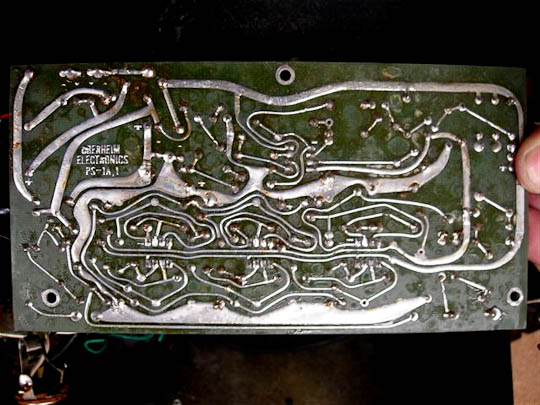
\includegraphics[width=2.5in]{hand-pcb.jpg}
\caption{A vintage PCB laid out by hand. Source: \href{http://grantmuller.com/maestro-ps-1b-teardown/}{Link}.}
\label{fig:hand-pcb}
\end{figure}

In recent years, \href{http://www.kicad-pcb.org/}{KiCad} has emerged as a popular open-source software package for designing and laying out PCBs. KiCad is available on all three major personal computer operating systems. Compared with the above mentioned software packages, KiCad is completely free of charge or any other limitation. Although KiCad is not as sophisticated as industry-level tools, it is capable of dealing with fairly complicated designs, and the active developer community is working hard to improve its capabilities. In fact, as of this writing, KiCad has not had an official stable release for the last two years because of the constant development progress being made. In this tutorial, we will be using the \href{http://kicad-pcb.org/download/windows/}{2015 stable release candidate 4.0.0 RC1}.

This tutorial will provide an introduction on how to use KiCad for PCB designs through two examples. 

\newpage
\section{Example 1: Arduino dice}
%TODO: add more description of the project 
In the first example we will make an eletronic dice consisting of an ATmega328P microcontroller\footnote{The heart of the Arduino UNO platform.}, a push-button switch, a 7-segment LED display, and some misc resistors and capacitors. Every time you press and release the switch, the microcontroller will generate a random number (1--6) for the dice value and display it on the 7-segment LED. This example is a stripped down version of \href{http://www.princetronics.com/electronic-dice/}{a project from PrinceTronics}. 

Table.~\ref{tab:example1} lists the components that are needed for this example.

\begin{table}[h]
\centering
\caption{List of components for Example 1.}
\begin{tabular}{|c|c|c|}
\hline \textbf{Item Description} & \textbf{Quantity} & \textbf{Digikey Part \#} \\ 
\hline \hline  Arduino Uno board, DIP version & 1 & \href{http://www.digikey.com/product-detail/en/A000066/1050-1024-ND/2784006}{1050-1024-ND} \\ 
\hline  16-MHz crystal oscillator &  1 & \href{http://www.digikey.com/product-search/en?KeyWords=300-8499-ND}{300-6034-ND} \\ 
\hline  22-pF ceramic capacitor, SMD, 0603, 5\% & 2 & \href{http://www.digikey.com/product-detail/en/C1608C0G1H220J080AA/445-1273-1-ND/567670}{445-1273-1-ND}  \\ 
\hline  1-uF ceramic capacitor, SMD, 0603 & 1 & \href{http://www.digikey.com/product-detail/en/CL10F105ZP8NNNC/1276-1041-1-ND/3889127}{1276-1041-1-ND}  \\ 
\hline  10k-Ohm resistor, SMD, 0603, 1/10W, 5\% & 2 & \href{http://www.digikey.com/product-detail/en/ERJ-3GEYJ103V/P10KGCT-ND/134717}{P10KGCT-ND} \\ 
\hline  Push button switch, 0.05 A, 24 V  & 1 & \href{http://www.digikey.com/product-search/en?KeyWords=SW400-ND}{SW400-ND} \\ 
\hline  7-segment 1-digit display, 
common cathode & 1 & \href{http://www.digikey.com/product-detail/en/HDSP-313E/516-2734-ND/2219051}{516-2734-ND} \\ 
\hline 
\end{tabular} 
\label{tab:example1}
\end{table}

\subsection{Starting KiCad}

Fig.~\ref{fig:kicad-main} shows the main window of KiCad. The main window serves as a project management panel where you can launch the individual PCB tools. Table.~\ref{tab:kicad-icons} lists the icons and descriptions of the KiCad tools. 

\begin{figure}[ht]
\centering
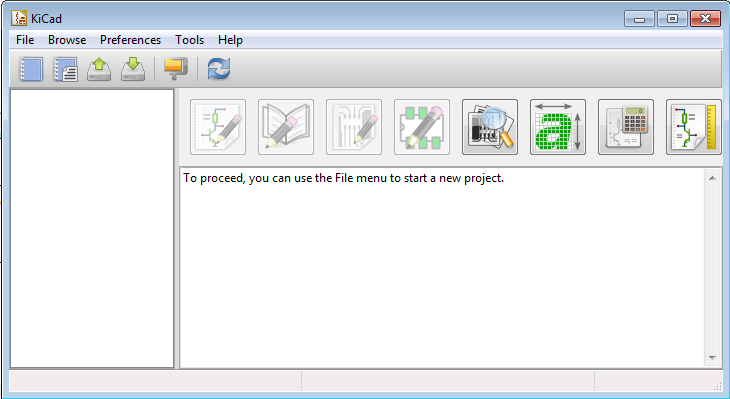
\includegraphics[width=4.5in]{kicad-main.png}
\caption{The main window of KiCad.}
\label{fig:kicad-main}
\end{figure}

\begin{table}[h]
\caption{Individual tools within KiCad.}
\begin{tabular}{|m{0.5in}|m{2in}||m{0.5in}|m{2in}|}
\hline 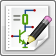
\includegraphics[width=0.5in]{eeschema-icon}  &   Eeschema: schematic editor/capture tool & 
\includegraphics[width=0.5in]{gerbview-icon} &  Gerbview: Gerber file viewer\\ 

\hline 
\includegraphics[width=0.5in]{sche-lib-icon} &  Schematic library editor & 
\includegraphics[width=0.5in]{bitmap2component-icon} &  Bitmap2Component: A tool for converting bitmap images to Eeschema or Pcbnew elements\\ 

\hline 
\includegraphics[width=0.5in]{pcbnew-icon} &  Pcbnew: PCB layout tool & 
\includegraphics[width=0.5in]{calculator-icon} &  A calculator for common PCB design related calculations\\ 

\hline 
\includegraphics[width=0.5in]{footprint-lib-icon} &  PCB footprint editor & 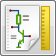
\includegraphics[width=0.5in]{pi-editor-icon} &  Worksheet sheet layout editor\\ 
\hline 
\end{tabular}
\label{tab:kicad-icons} 
\end{table}


\newpage
\subsection{Schematic Capture}

\begin{enumerate}
	\item Click on the ``Create New Project'' button to create a new project and name it ``arduino\_dice.pro''.
	\item Click on the Eeschema icon. A new schematic window should appear.
	\item Save your schematic design with the file name ``arduino\_dice.sch''. 
	\item The default library that comes with KiCad installation has schematic symbols for many ATmel micro-controllers, including the ATmega328P that is used on the Arduino platform. You can place the symbol on your schematic by the following steps. 
		\begin{enumerate}
			\item Click on the ``Place a component'' button from the toolbar on the right side. Fig.~\ref{fig:eeschema-toolbar} shows a list of Eeschema toolbar buttons, their functions, and the corresponding keyboard shortcuts. 
			
				\begin{figure}[hp]
					\centering
					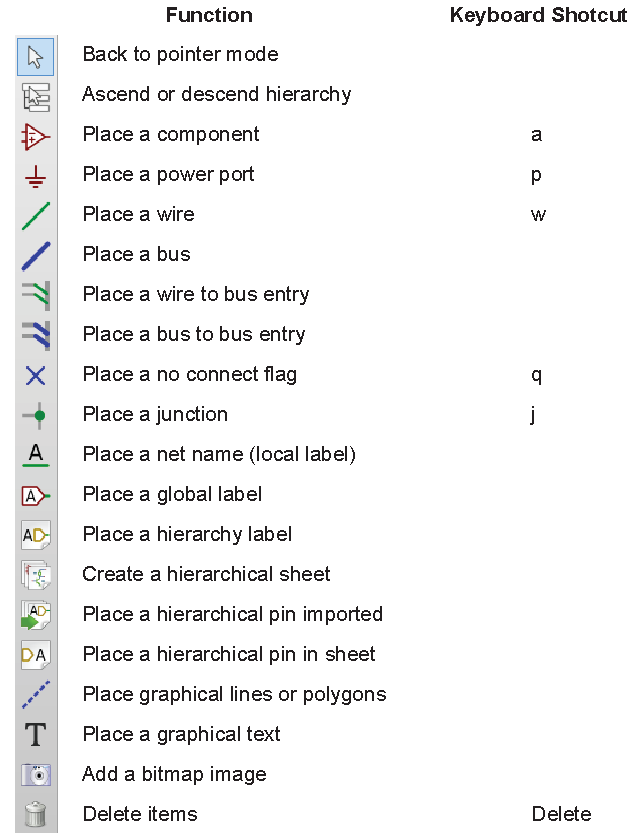
\includegraphics[width=5in]{eeschema-toolbar}
					\caption{Eeschema toolbar icons.}
					\label{fig:eeschema-toolbar}
				\end{figure}
				
			\item Click anywhere on the schematic, a dialog box should appear (Fig.~\ref{fig:place-component}). 
				\begin{figure}[hp]
					\centering
					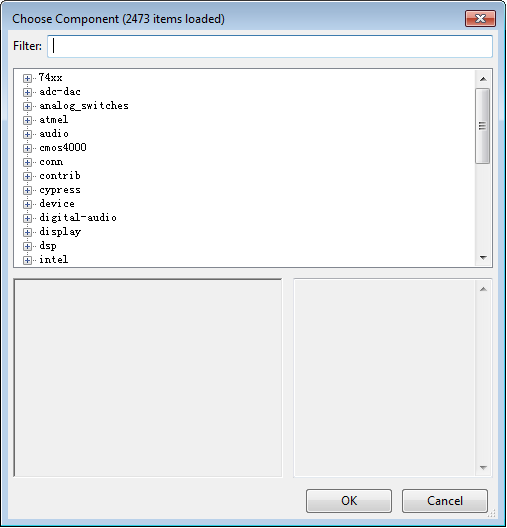
\includegraphics[width=3in]{place-component.png}
					\caption{Place component dialog box.}
					\label{fig:place-component}
				\end{figure}

			\item We'll add our first item, the ATmega328P microcontroller, from the ``atmel'' library. Select the ``atmel'' entry, and click ``OK''. A new dialog box appears for you to select the particular device, the “ATMEGA328P-P”. Click ``OK''. Note that if you already know the name of the component, you can simply start typing the name and Eeschema will filter out the components with the same initial characters. It wouldn't take long before you arrive at your desired component.
			
			\item The ATmega328P symbol should now cling to your mouse cursor. Click on the schematic to place it at a location you like. 
			\item A number of component editing operations are available by right clicking on the component (Fig.~\ref{fig:edit-component}). Some of the operations have keyboard shortcut. The general way to use the shortcut is to place the cursor on the component and press the corresponding shortcut key. Pressing the ``ESC'' key will cancel the current operation. 
			
			\begin{figure}[h]
				\centering
				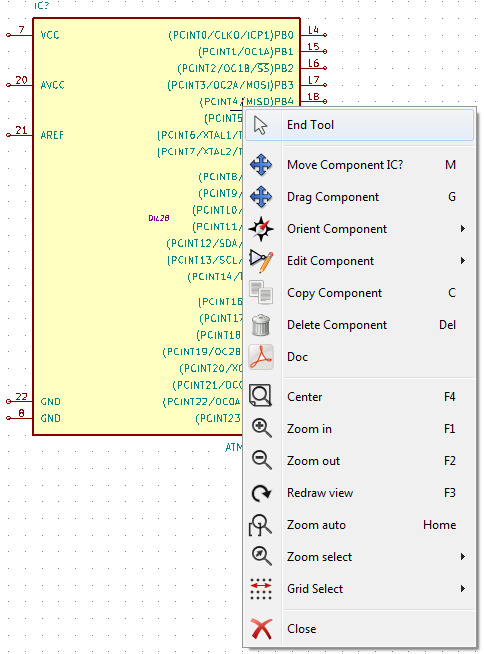
\includegraphics[width=3in]{edit-component}
				\caption{Edit component pop-up menu.}
				\label{fig:edit-component}
			\end{figure}

				\begin{enumerate}
					\item ``Move component'' will move the component and break all circuit connections to it. To retain the connections, use ``Drag component''. 
					\item ``Orient component'' has further options to rotate and mirror the component. Experiment the shortcuts by pressing ``r'' or ``y'' while placing the cursor on the component.
					\item ``Edit component$\rightarrow$ Edit'' will bring up a dialog box that allows you to edit all of the component properties. 
						\begin{enumerate}
							\item The ``Reference'' and ``Value'' are the two properties that you are most likely to edit in this dialog box. ``Reference'' is the annotation of the component. In this case, it should read ``IC1''. You may also write it as ``IC?'' where the ``?'' is a placeholder for a numeric value. KiCad can auto annotate the components and assign a unique value for each component; we will look at how to do this shortly.
							\item The ``Value'' entry is usually used to mark the component value. For resistors, capacitors, and inductors, the ``Value'' can simply be their corresponding resistance, capacitance, and inductance values. For this ATmega microcontroller we will simply use the ``Value'' to mark the component’s name. 
							\item For now, we will delete the value for the ``Footprint'' field. 
						\end{enumerate}
				\end{enumerate}
		\end{enumerate}

	\item Follow a similar procedure to place the other circuit components. Table.~\ref{tab:example1-sche} lists which library they belong to and their names in the library. 
	
	Note that the VCC and GND symbols, and all other symbols related to providing power to the circuits, are organized into the \emph{power} library. They can be accessed directly by clicking the ``Place a power port'' button from the toolbar on the right. 
	
		\begin{table}[ht]
			\centering
			\caption{Schematic components for Example 1.}
			\renewcommand{\arraystretch}{1.2}
			\begin{tabular}{|c|c|c|c|}
			\hline \textbf{Component} & \textbf{Library} & \textbf{Name in Library} & \textbf{Value} \\
			\hline 
			\hline ATmega328P & atmel & ATMEGA328P-P & \\
			\hline Two 22-pF capacitors & device & C & 22\,pF \\ 
			\hline One 1-uF capacitor & device & C & 1\,uF \\ 
			\hline One 16-MHz crystal oscillator & device & CRYSTAL & 16\,MHz \\ 
			\hline One 7-segment LED display & display & 7SEGMENTS &  \\ 
			\hline One push button & device & SW\_PUSH &  \\ 
			\hline Two 10-k resistors & device & R & 10\,k \\ 
			\hline 2-pin header &  conn & CONN\_01X02 &  \\ 
			\hline Vcc & power & vcc &  \\ 
			\hline Ground & power & GND &  \\ 
			\hline 
			\end{tabular}
			\label{tab:example1-sche}
		\end{table}
	\item Connect the components together according to Fig.~\ref{fig:example1-schematic-1} by placing wires between corresponding pins. The components should be arranged to make connecting them together easier with less wire clutter. To start placing a wire, click on the ``Place a wire'' button, then click on the starting point, and finish by clicking on the endpoint of the wire. It is often easier to use the keyboard shortcut. First move your cursor to the starting point and press the ``w'' key. A wire will be started at the cursor location. Move the cursor to the endpoint and click to finish the connection. 
	
		\begin{figure}[h]
			\centering
			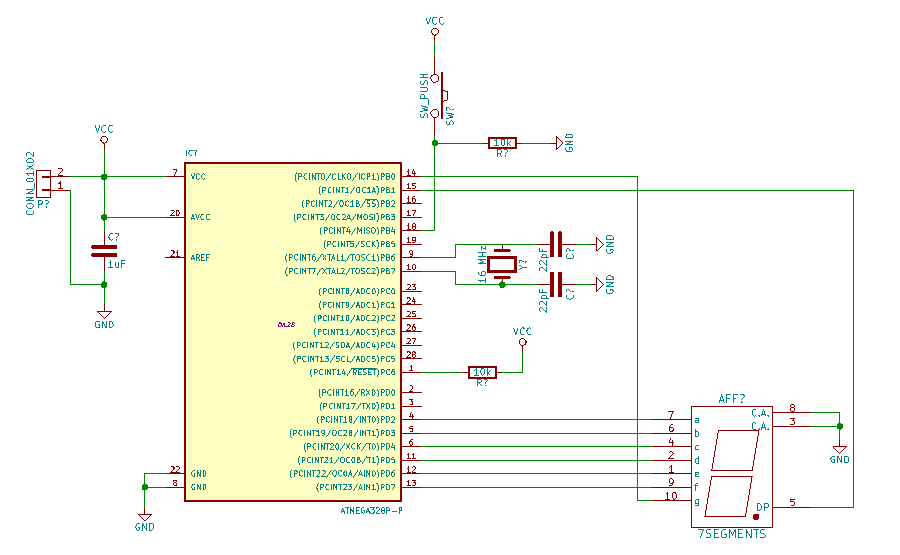
\includegraphics{example1-schematic-1}
			\caption{Initial schematic drawing of Example 1 circuit.}
			\label{fig:example1-schematic-1}
		\end{figure}
	
	\item The schematic can become difficult to read if there are too many wire crossovers. ``Named netlist'' can be used to alleviate the issue. Although our example circuit is quite simple, we will still use it to illustrate how to ``clean up'' the schematic with named net.
		\begin{enumerate}
			\item Delete the wire between the ATmega328P's PB1 pin and the 7-segment LED's DP pin. 
			\item Draw a short section of wire on the ATmega328P's PB1 pin; one of the ends of the wire is now floating. 
			\item Click the ``Place a net name -- local label'' button and then click on the schematic. A dialog box will appear, input ``DP'' in the ``Text'' field, and click ``OK''. The text ``DP'' can now be seen to cling on the cursor. 
			\item Click on the floating terminal of the short wire on the PB1 pin to finish naming the net. You should now see the text ``DP'' attached to the wire on the PB1 pin; the little hollow square at the floating end of the wire has also disappeared. 
			\item Repeat steps b--d for the DP pin of the 7-segment LED. The ATmega328P's PB1 pin and the 7-segment LED's DP pin are now connected by the net name ``DP'' even though there is no direct wire connection on the schematic view. 
			\item Repeat steps a--e for the connection between ATmega328P's PB4 pin and the push button. Refer to the final schematic (Fig.~\ref{fig:example1-schematic-final}) for how it looks.  
		\end{enumerate}
	
	\item In most circuits, the unused pins can be left floating. In this example, however, we will terminate all the unused pins by placing a ``no connect'' label on them; this tells KiCad to ignore these pins during the electrical rule check (ERC).
	
	\item The schematic capture is now almost done. Notice that the references to some of the components still have question marks. For example, the two capacitors connected to the crystal oscillator look identical to each other. We need to differentiate them. In KiCad, we do this by \textit{annotating} the schematic, i.e. giving each component a unique identifier (reference). Annotation can be done manually by changing the ``Reference'' property of a component and making sure that each reference is unique, but it is much easier to let KiCad do the annotation automatically. Here is how:
		\begin{enumerate}
			\item Click the ``Annotate'' button. 
			\item A dialog box appears. The options are all self-explanatory. 
		
			\item Click the ``Annotate'' button to finish. You must have noticed that you can ``un-annotate'' the schematic by clicking the ``Clear annotation'' button. 
			
			\item After annotation, you should see that all the components are now numbered properly. 
		\end{enumerate}
		
	\item It is always a good idea to run an ERC. ERC checks the electrical connections between components and try to detect potential errors in the schematic. In KiCad, you can do this by clicking the ERC button. 
	
	\item Once you've passed the ERC, generate a netlist by clicking the ``Generate netlist'' button. This will create a netlist file that describes the circuit connections. The netlist file will be used to guide the PCB layout process.
	
	\item The final schematic should look like that in Fig.~\ref{fig:example1-schematic-final}.
		\begin{figure}[h]
			\centering
			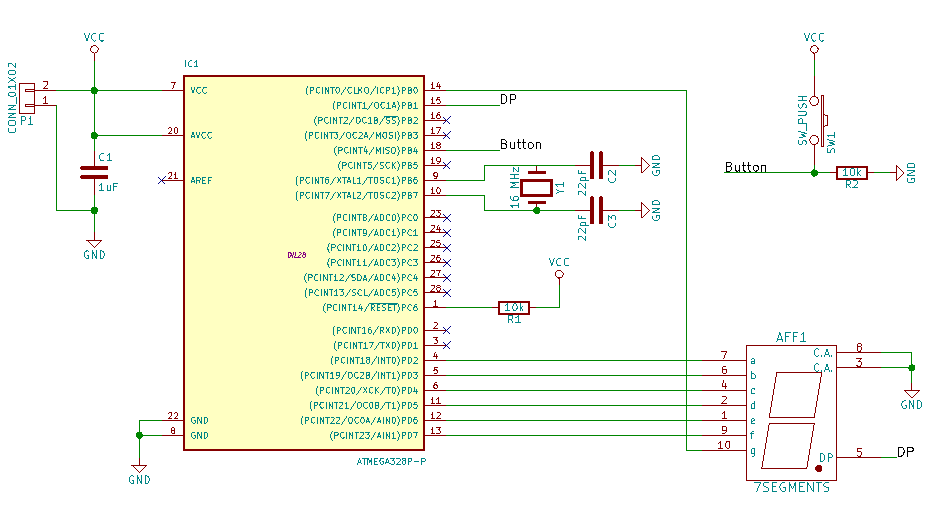
\includegraphics{example1-schematic-final}
			\caption{Completed schematic drawing of Example 1 circuit.}
			\label{fig:example1-schematic-final}
		\end{figure}		
\end{enumerate}

\newpage
\subsection{Creating Schematic Symbols}
%TODO: add discussion on the selection of grid size; the grid is like a breadboard
Sometimes you run into a situation where you cannot find a proper schematic symbol in the default KiCad library for the component that you want to use. The following steps will show you how to create a schematic symbol of your own. 

\begin{enumerate}
	\item From the KiCad project window, click the ``Schematic library editor'' button to launch the schematic symbol editor and library manager. The library editor window should appear. Alternatively, you can launch it by clicking the same button from Eeschema.
	
	\begin{figure}[h]
		\centering
		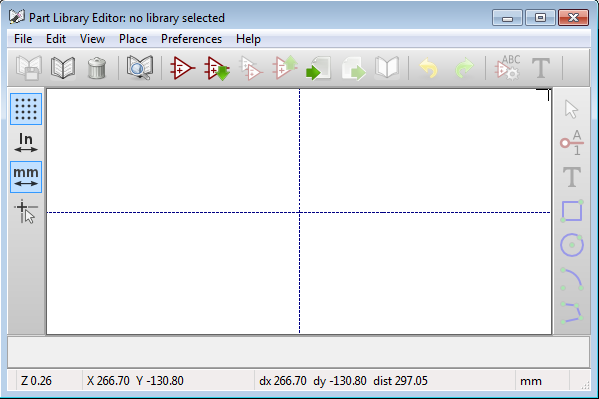
\includegraphics[width=0.6\linewidth]{sche-lib-editor}
		\caption{The schematic library editor program}
		\label{fig:sche-lib-editor}
	\end{figure}
	
	\item Click the ``Select working library'' button to set the current working library. A dialog box should appear with the same list of component libraries that we saw when we placed components on the schematic. 
		\begin{enumerate}
			\item If you are creating a new component, it is recommended that you select the project library, which is by default named ``\textit{project\_name}-cache'' and should be the last one in the list. In this example, select the library named ``arduino\_dice-cache''. 
			
			\item If you are trying to edit an existing component, click the corresponding library.
			
			\item Click ``OK'' to finalize the selection. 
		\end{enumerate}
	
	\item In this example, we are actually not missing any schematic symbol. Just for the sake of demonstrating how to use the library editor, we will build our own version of the ATmega328P microcontroller IC. Fig.~\ref{fig:atmega328p-pins} shows the pin diagram of the ATmega328P.
		\begin{figure}[hp]
			\centering
			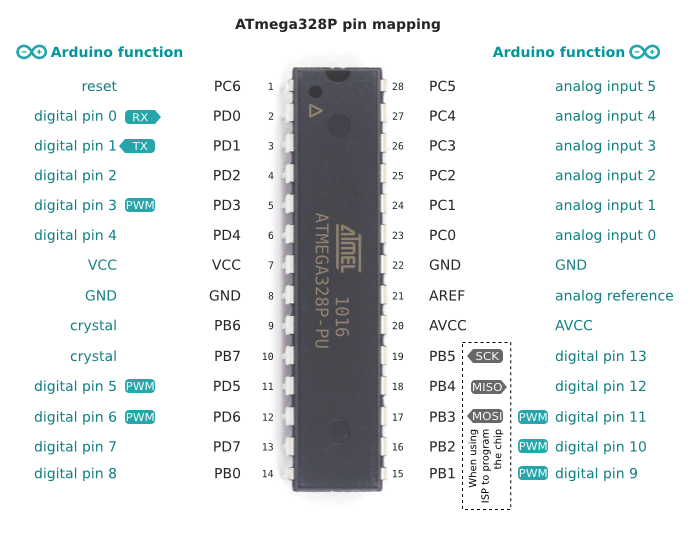
\includegraphics[width=5in]{atmega328p-pins}
			\caption{Pin mapping for the ATmega328P microcontroller. Source: \href{https://www.pinterest.com/pin/401101910534454835/}{Link}.}
			\label{fig:atmega328p-pins}
		\end{figure}

	\item Click the ``Create a new component'' button. A dialog box will appear (Fig.~\ref{fig:create-component}). Put \nohyphens{``ATmega328p''} as the component name. Leave everything else as default. Worth mentioning is the ``Number of parts per package'' setting. Sometimes a component may have many pins and it becomes difficult to route the schematic (or to be more precise, it becomes difficult to read the schematic when you have lots of wire connections). In this case, it may be easier to split a component into several schematic symbols so that routing can be easier. In such a scenario, you can have multiple parts per package. 
		\begin{figure}[hp]
			\centering
			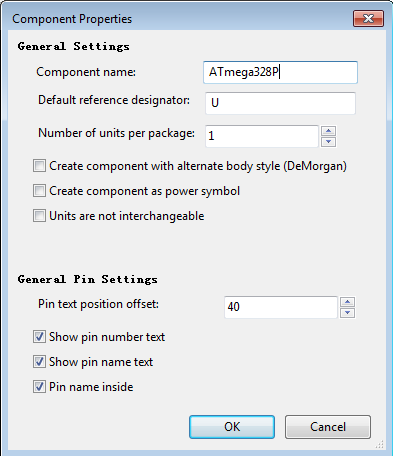
\includegraphics[width=3in]{create-component}
			\caption{Creat component dialog box.}
			\label{fig:create-component}
		\end{figure}
		
	\item Click ``OK'' and you should see the component ``Reference'' and ``Value'' strings appearing near the center of the library editor main window. 
	
	\item Click the ``Add graphic rectangle to the component body'' button , and use the mouse cursor to draw a rectangle from $(x=-0.400'', y=0.700'')$ to $(0.400'',-0.700'')$ (Fig.~\ref{fig:draw-rectangle-symbol}). The current position of the cursor is displayed in the status bar at the bottom of the main window. Notice that the positive direction of the $y-$axis points downward. 
		\begin{figure}[h]
			\centering
			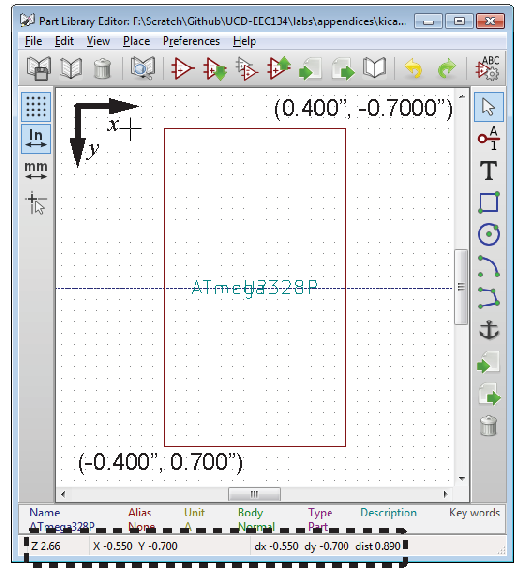
\includegraphics{draw-rectangle-symbol.pdf}
			\caption{Drawing a rectangle in the library editor main window with the help of the built-in cordinate system.}
			\label{fig:draw-rectangle-symbol}
		\end{figure}
		
	\item Add component pins. 
		\begin{enumerate}
			\item Click the ``Add pins to the component'' button 
			
			\item Click anywhere in the main drawing window. A dialog box should appear. Put ``PC6'' for the ``Pin name'', ``1'' for the ``Pin number'', ``Right'' for the ``Orientation'', ``Input'' for the ``Electrical type'', and leave everything else as default. 
			
			\item Click ``OK'', and then click at $(-0.600, -0.650)$ to add the pin. 
		\end{enumerate}

	\item Repeat the above process and add the rest of the pins as follows. 
		\begin{table}[hp]
			\centering
			\begin{tabular}{|p{0.5in}|p{0.5in}|p{0.5in}|p{1in}||p{0.5in}|p{0.5in}|p{0.5in}|p{1in}|}
				\hline  \textbf{Pin Name} & \textbf{Pin number} & \textbf{Orien-tation} & \textbf{Electrical Type} & \textbf{Pin Name} & \textbf{Pin number} & \textbf{Orien-tation} & \textbf{Electrical Type}\\ 
				\hline \hline PD0 & 2 & Right & Input & PC5 & 28 & Left & Input\\ 
				\hline PD1 & 3 & Right & Input & PC4 & 27 & Left & Input\\ 
				\hline PD2 & 4 & Right & Input & PC3 & 26 & Left & Input \\ 
				\hline PD3 & 5 & Right & Input & PC2 & 25 & Left & Input\\ 
				\hline PD4 & 6 & Right & Input & PC1 & 24 & Left & Input\\ 
				\hline VCC & 7 & Right & Power Input & PC0 & 23 & Left & Input\\ 
				\hline GND & 8 & Right & Power Input & GND & 22 & Left & Power Input\\ 
				\hline PB6 & 9 & Right & Input & AREF & 21 & Left & Input\\ 
				\hline PB7 & 10 & Right & Input & AVCC & 20 & Left & Power Input\\ 
				\hline PD5 & 11 & Right & Input & PB5 & 19 & Left & Input\\ 
				\hline PD6 & 12 & Right & Input & PB4 & 18 & Left & Input\\ 
				\hline PD7 & 13 & Right & Input & PB3 & 17 & Left & Input\\ 
				\hline PB0 & 14 & Right & Input & PB2 & 16 & Left & Input\\ 
				\hline & & & & PB1 & 15 & Left & Input\\
				\hline 
			\end{tabular} 
		\end{table}
	
	\item Now move the ``Reference'' string above the rectangle (only for aesthetic reasons) and the ``Value'' string below the rectangle. You can also add a half circle (arc) to the top of the rectangle to indicate the orientation of the component. Fig.~\ref{fig:atmega328p-symbol-final} shows the completed component symbol. 
		\begin{figure}[h]
			\centering
			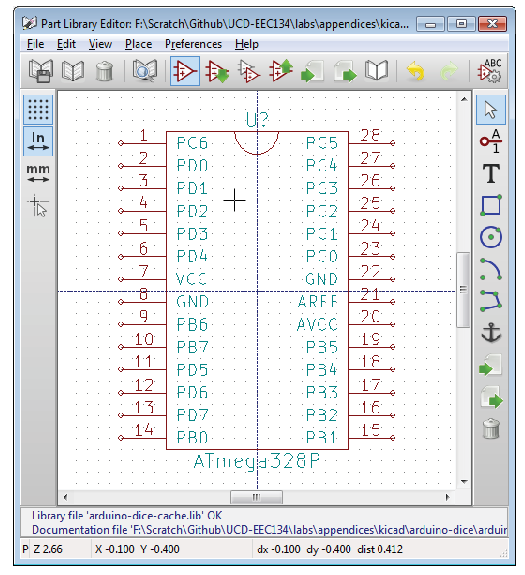
\includegraphics{atmega328p-symbol-final.pdf}
			\caption{Completed schematic symbol for the ATmega328P microcontroller.}
			\label{fig:atmega328p-symbol-final}
		\end{figure}
		
	\item Click the “Save current library to disk” to save your work. This should complete the creation of the schematic symbol. To verify that you have successfully created the symbol, go back to the Eeschema window and check whether you can find the ATmega328P symbol you just built in the ``arduino-dice-cache'' library. 
	
\end{enumerate}

\newpage
\subsection{Associating schematic symbols with footprint}
\label{sec:cvpcb}

In KiCad, the schematic symbol and the footprint of a device are stored in separate files (.lib for schematic symbols and .mod for footprint). In order for the PCB layout tool (Pcbnew) to put the correct footprints in the layout, we need to establish a relationship between the schematic symbols and the footprints in a circuit. The CvPcb program is used to do this in KiCad. 

\begin{enumerate}
	\item Open CvPcb from the Eeschema window. By default, CvPcb should automatically loaded the netlist of the project. If not, you can go to ``File$\rightarrow$Open'' to open the desired netlist. Ignore any error messages at this stage.
	
	\item The CvPcb window consists of three panes. The leftmost one lists the footprint libraries. The center one lists all the schematic components used in the circuit. The right one presents a list of available footprints. These footprints are installed with the KiCad program. By default, CvPcb presents only footprints that it thinks that are relevant to the components. To see a full list of available components, uncheck the ``Filter footprint list by keywords'' button. 
	
	\item Our job in CvPcb is to associate the schematic components with their corresponding footprint. This is done by first selecting the component in the middle pane, and then double clicking on the right footprint in the right pane. You can preview the drawing of the footprint by clicking the ``View selected footprint'' button . 
	
	\item \textbf{A very important rule in PCB design is to never trust footprints provided by others unless 1) they are directly from the component vendors; 2) you have verified them yourself.} The default footprint library that comes KiCad is particularly error prone. For this reason, we will be creating all the footprints by ourselves in this example. The next section outlines this process. 
\end{enumerate}

\subsection{Creating or Editing Footprint}
%TODO: add discussion of the different layers created in the footprint editor. 
%e.g.: solder mask clearance: https://forum.kicad.info/t/insufficient-soldermask-clearance/144

\subsubsection{SMD capacitor}
\label{sec:smd_cap_footprint}

We will start with the simplest component in the circuit, the 22-pF capacitor. This capacitor is a 0603 SMD capacitor produced by TDK Corporation. ``0603'' refers to its lateral dimensions in thousandth of an inch (normally referred to as a \textbf{mil} or a \textbf{thou}), that is, the capacitor is roughly 60-mil long and 30-mil wide. If we look at the dimension drawing provided by the vendor (Fig.~\ref{fig:tdk_cap_datasheet}-a), we see that its actual dimensions are 63\,mil$\times$31\,mil. In fact, the capacitor is realy sized in the metric system, with a nominal dimension of 1.6\,mm$\times$0.8\,mm. So this capacitor is a ``0603'' in imperial units and ``1608'' in metric units. \textbf{The difference between the imperial and metric units is a common source of confusion when choosing components. Always double check!}

On the \href{http://www.digikey.com/product-detail/en/C1608C0G1H220J080AA/445-1273-1-ND/567670}{Digikey product page}, we can find the datasheet to the capacitor \href{http://product.tdk.com/en/catalog/spec/mlccspec_commercial_general_midvoltage_en.pdf}{``C Series, Gen Appl \& Mid-Voltage Spec''}. Page 15 of the datasheet, copied here in Fig.~\ref{fig:tdk_cap_datasheet}-b, shows the recommended land pattern (footprint) for the capacitors in this serie of products. The recommended dimensions for the 0603 (1608 metric) capacitor is highlighted. Here we will use the median value of 0.7\,mm for A, B, and C. 

	\begin{figure}[hp]
		\centering
		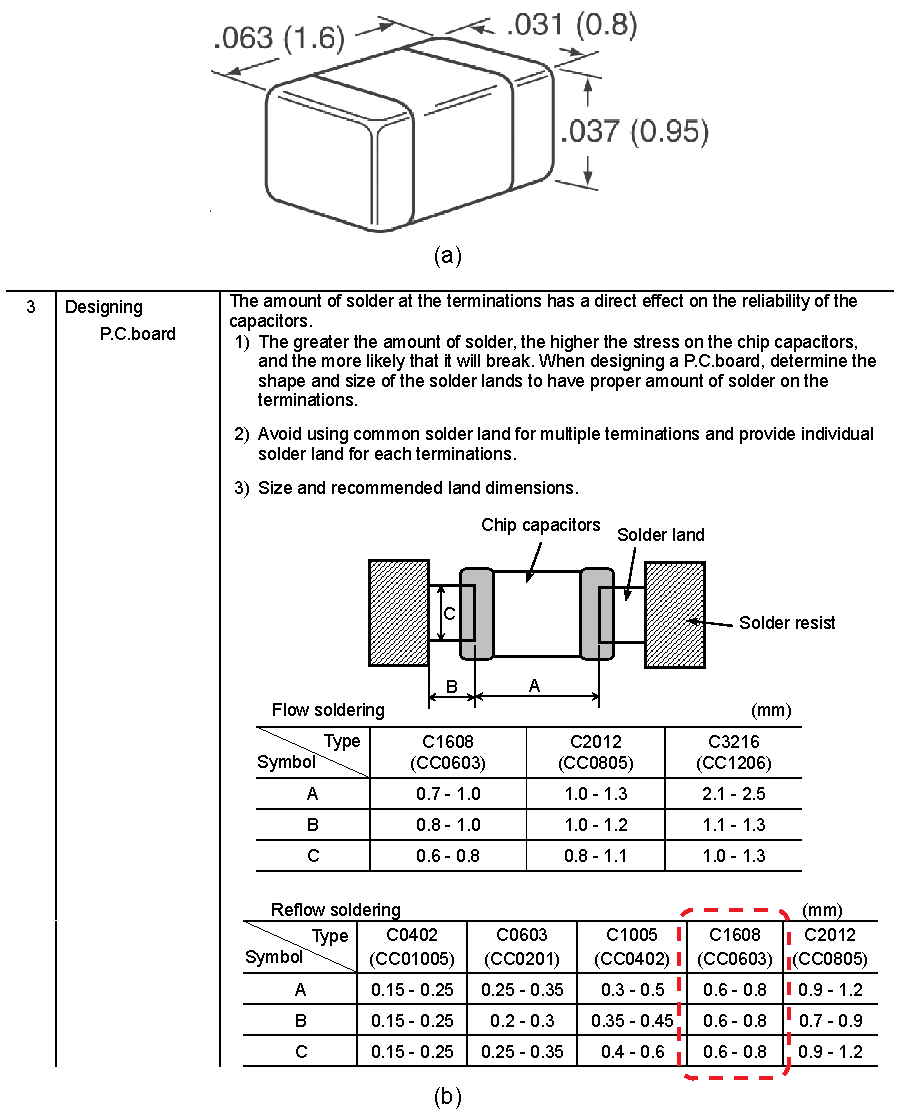
\includegraphics{tdk_cap_datasheet}
		\caption{(a) Dimensions of the TDK C-series 22-pF SMD capacitors. (b) PCB design recommendation for TDK C-series SMD capacitors. Land pattern dimensions for the C1608 type is highlighted in red.}
		\label{fig:tdk_cap_datasheet}
	\end{figure}

Now let's start drawing the footprint for the capacitor. 
\begin{enumerate}
	\item Start the PCB footprint editor by clicking on the ``PCB footprint editor'' button. 
	
	\item Click the ``New footprint'' button to create a new footprint. Put ``smd\_0603'' as the name in the pop-up dialog box. Click ``OK''. 
	
	\item By default, the footprint name ``smd\_0603'' and the Reference string ``REF**'' will appear in the center of the drawing window. 
	
	\item Set the working unit to ``mm'' (millimeters). Then set the grid size to ``User grid''. The user grid size can then be set by going to menu ``Dimensions$\rightarrow$User Grid Size''. Set the unit to ``Millimeters'', ``Size X'' to ``0.05'', and ``Size Y'' to ``0.05''.
	
	\item Click the ``Add pads'' button. Move the cursor to position (-0.7, 0) and click. A donut-shape patch should appear. This is because by default KiCad assumes a through-hole type pad. 
	
	\item To change the pad properties, move the cursor on top of the pad and type keyboard short ``e'' for editing. The \emph{Pad Properties} dialog box should appear. Change the properties as follows:
		\begin{table}[h]
			\centering
			\caption{Pad properties for the SMD capacitor.}
			\renewcommand{\arraystretch}{1.2}
			\small
			\begin{tabular}{|c|c|}
				\hline  Pad number & 1 \\ 
				\hline  Pad type & SMD \\ 
				\hline  Shape & Rectangular shape \\ 
				\hline  Position X & -0.7 \\ 
				\hline  Position Y & 0  \\ 
				\hline  Size X & 0.7 \\ 
				\hline  Size Y & 0.7  \\ 
				\hline  Layers & F.Cu \\ 
				\hline  Technical Layers & Check ``F.Paste'', ``F.SilkS'', and ``F.Mask''  \\ 
				\hline 
			\end{tabular} 
		\end{table}
	
	\item Repeat Step 5 and 6 to add the second pad at the correct location. You will notice that KiCad assumes the properties of the previous pads as the default properties of the new pad. 
	
	\item Draw the courtyard outline of the capacitor using ``Add graphic line or polygon'' tool. The courtyard is the actual dimension of the device plus some margin. It serves as a guide to prevent the PCB designer from placing components too close to each other. Here we have put a decent margin of 0.45\,mm in the $x $-direction and 0.65\,mm in the $y$-direction around the pads (or 0.7\,mm in $x$ and 0.6\,mm in $y$ around the component). This margin can be adjusted according to the assembly requirement and tolerances in the PCB assembly process.  
	  
	\item The finished footprint drawing should look like that shown in Fig.~\ref{fig:smd_cap_footprint_final}.
		
		\begin{figure}[hp]
			\centering
			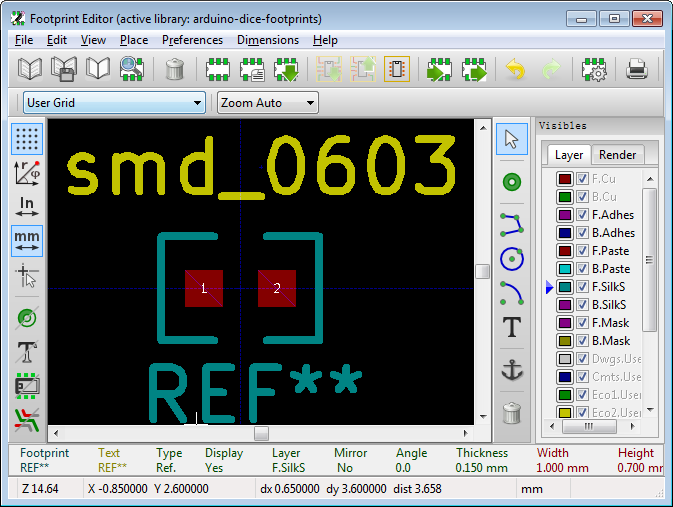
\includegraphics[width=3in]{smd_cap_footprint_final}
			\caption{Completed footprint of the SMD 0603 capacitor.}
			\label{fig:smd_cap_footprint_final}
		\end{figure}
			
	\item We wish to create a new library to contain our newly created footprint. To do this, click the ``Create new library and save current module'' icon. Set the location and name of the library and click ``OK''. The ``Library Path'' field should contain the full path to your desired library location. In this example, we will create a footprint library with the name ``arduino-dice-footprints'' (KiCad will automatically add the ``.pretty'' suffix) under the project folder ``...$\backslash$arduino-dice''. Fig.~\ref{fig:create-new-footprint-library} shows the proper settings. A new folder named ``arduino-dice-footprints.pretty'' should appear in the project tree in the KiCad main window (Fig.~\ref{fig:kicad-footprint-library}). Click on the ``$+$'' sign will expand the library and show all the footprints in this library. At this point, we only have the ``smd\_0603'' footprint.
	
		\begin{figure}[hp]
			\centering
			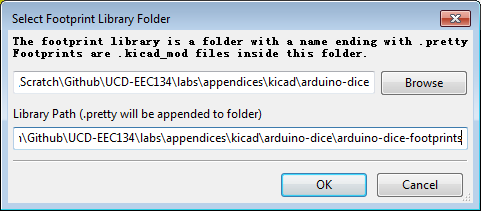
\includegraphics{create-new-footprint-library}
			\caption{The ``Select Footprint Library Folder'' dialog box.}
			\label{fig:create-new-footprint-library}
		\end{figure}

		\begin{figure}[hp]
			\centering
			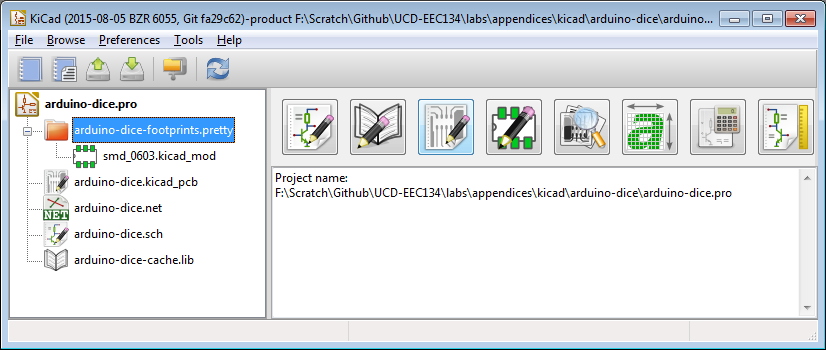
\includegraphics[width=4.5in]{kicad-footprint-library}
			\caption{The new footprint library is now visible in the project tree.}
			\label{fig:kicad-footprint-library}
		\end{figure}
	
	\item Although we now have the new footprint library in our file system and the project tree, KiCad still does not recognize it as part of the available libraries that we can pull footprints from. We will need to manually add the library to KiCad's \emph{library tables}. 
		\begin{enumerate}
			\item 	Open CvPcb and click the ``Edit footprint library table'' icon. The ``PCB Library Tables'' dialog box should appear. 
			
			\item Click the ``Append with Wizard'' button.
			
			\item In the pop-up dialog box, select ``Files on my computer'' and click ``Next''. 
			
			\item Browse to and select the footprint library folder we just created, click ``Next''. Click ``Next'' again in the next window to confirm. 
			
			\item Select ``To the current project only'' and click ``Finish'' to finish adding the footprint library to this project. If you have created a generic library that you want to use across multiple projects, you could select the ``To global library configuration'' option. Fig.~\ref{fig:add-project-footprint-lib} shows how the ``PCB Library Tables'' looks like now. Notice how KiCad replaces the absolute path with the ``KIPRJMOD'' environment variable. 

					\begin{figure}[hp]
						\centering
						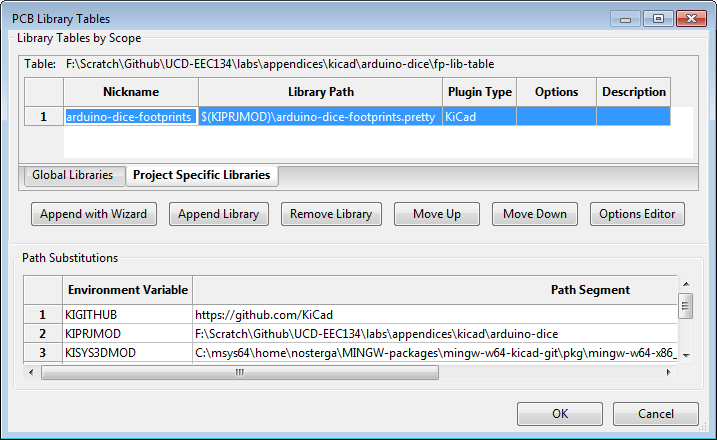
\includegraphics[width=5in]{add-project-footprint-lib}
						\caption{Add a project footprint library.}
						\label{fig:add-project-footprint-lib}
					\end{figure}
					
			\item Finally, if you plan to create more footprints, it's a good idea to set the active library in the Footprint Editor. In the Footprint Editor window, click the ``Set active library'' icon, select the ``arduino-dice-footprints'' library which should be at the bottom of the list, and then click ``OK''.  
		\end{enumerate}
	
\end{enumerate}

\subsubsection{Push button switch}
\label{sec:sw_footprint}
The Omron B3F-1000 push botton switch is a through-hole component. Page 225 of its datasheet shows the detailed dimensions of the device (Fig.~\ref{b3f-datasheet}) and can be used to guide the footprint design.  

	\begin{figure}[hp]
		\centering
		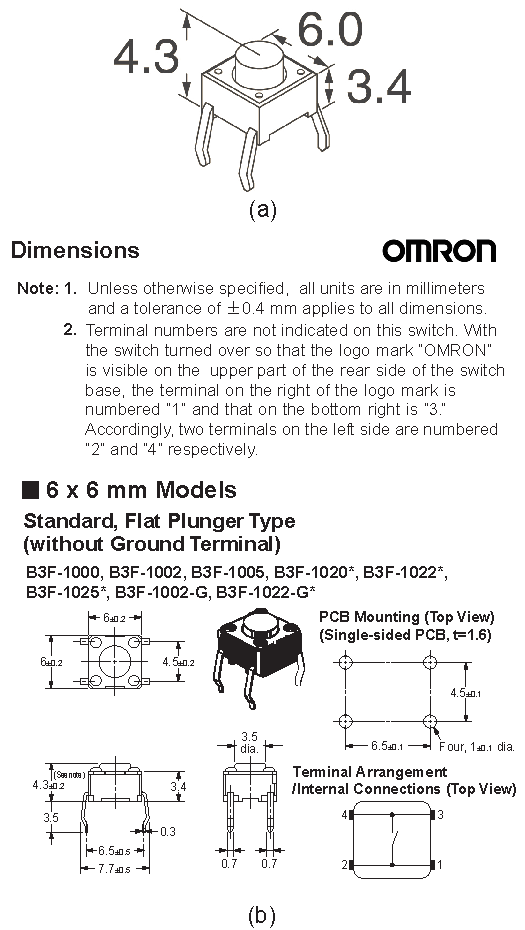
\includegraphics[width=3.5in]{b3f-datasheet}
		\caption{(a) Dimension drawing and (b) suggested footprint of the B3F-1000 switch.}
		\label{b3f-datasheet}
	\end{figure}

The footprint for the switch consists of four 1\,mm diameter holes spaced 6.5\,mm apart in the $x$-direction and 4.5\,mm apart in the $y$-direction. Use similar steps as in Sec.~\ref{sec:smd_cap_footprint} to create the switch footprint. Use the parameters in Table.~\ref{tab:pad-parameters} for the through hole pads. 
	\begin{table}[hp]
		\centering
		\caption{Parameters for through-hole pads for the B3F switch.}
		\renewcommand{\arraystretch}{1.2}
		\small
		\begin{tabular}{|c|c|}
			\hline  Pad type & Through-hole \\ 
			\hline  Shape & Circular shape \\ 
			\hline  Position X & $\pm$ 3.25 \\ 
			\hline  Position Y & $\pm$ 2.25  \\ 
			\hline  Size X & 2.032 (80\,mil) \\ 
			\hline Drill: Size X & 1 \\					 
			\hline  Layers & All copper layers \\ 
			\hline  Technical Layers & Check ``F.SilkS'', ``F.Mask'',  and ``B.Mask''  \\ 
			\hline 
		\end{tabular} 
		\label{tab:pad-parameters}
	\end{table}
			
Fig.~\ref{fig:switch-footprint-final} shows the completed footprint drawing for the switch. 

	\begin{figure}[h]
		\centering
		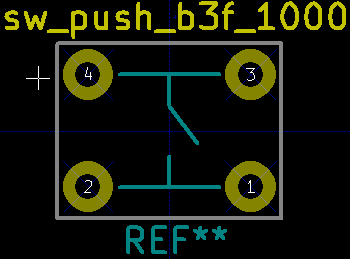
\includegraphics[width=2.in]{switch-footprint-final}
		\caption{Completed footprint for the Omron B3F-1000 push button switch.}
		\label{fig:switch-footprint-final}
	\end{figure}

\subsubsection{ATmega328P microcontroller}

The ATmega328P microcontroller powers the popular Arduino UNO platform. There are two variants of the UNO, one with the ATmega328P-PU which is a through hole package and the other with an SMD ATmega328P. In this example, we will be using the through-hole version (ATmega328P-PU) because it allows us to program the microcontroller on the UNO, unplug the microcontroller, and put it on our own PCB. 

The ATmega328P-PU uses a standard 0.3'' 28-pin dual inline package (28-DIP), i.e. there are two rows of pins with a 0.1'' pitch (distance between pins) and 0.3'' row spacing. We can follow the same procedures as in Sec.~\ref{sec:smd_cap_footprint} and \ref{sec:sw_footprint} to create its footprint, but this time we'll show you how to do it by modifying an existing footprint from the default KiCad library. 

\begin{enumerate}
	\item In Footprint Editor, click the ``Select active library'' button. In the pop-up dialog box, select the ``Sockets\_DIP'' library and click ``OK''. 
	
	\item Click the ``Load footprint from library''. In the pop-up dialog box, click ``List all''. In the component listing, click ``DIP-28\_300'', and then click ``OK''. The default 28-DIP package should appear in the Library Editor window.
	
	\item Verify that all the pads have the right dimensions (drill size, pitch and row spacing). 
	
	\item Hover the mouse cursor on top of (oftern called ``mouse over'') the string ``DIP-28\_300'' and change it to ``atmega328p-pu'' so that it's more recognizable when we do the layout later on. Fig.~\ref{fig:atmega328p-footprint-final} shows the completed footprint.
		\begin{figure}[hp]
			\centering
			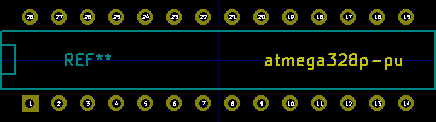
\includegraphics[width=3.55in]{atmega328p-footprint-final}
			\caption{Completed footprint for the ATmega328P-PU microcontroller.}
			\label{fig:atmega328p-footprint-final}
		\end{figure}
		
	\item Now click the ``Select active library'' icon and select the ``arduino-dice-footprints'' library. Click the ``Save footprint in active library'' icon to save the footprint in our project footprint library. 
\end{enumerate}

\subsubsection{The rest of the components}
Similar to the ATmega328P-PU microcontroller, the Avago HDSP-313E 7-segment LED display follows a standard 0.3'' 10-DIP pin arrangement. Therefore we can modify a standard 10-DIP footprint (Library: ``Sockets\_DIP$\rightarrow $DIP-10\_300'') for the 7-segment. Again, always double check all the dimensions if you are basing your work on someone else's footprint. Also notice that the 7-segment display has a much wider body than a typical 10-DIP IC. You will need to modify the courtyard and the silkscreen markings according to the \href{http://www.avagotech.com/docs/AV02-3585EN}{datasheet}. 

The footprint of the 16\,MHz crystal can be created manually from its \href{http://media.digikey.com/pdf/Data\%20Sheets/Citizen\%20PDFs/HC49US.pdf}{datasheet}. Given the practice we have done so far, it should be relatively straightforward to do. 

The 1-uF capacitor and the 10-k resistor are both 0603 components and they will share the same footprint as the 22-pF capacitor. Please DO double check their datasheets to verify that the same footprint can be used!

Fig.~\ref{fig:other-footprints-final} shows the footprints for the 7-segment display and the crystal. 
	\begin{figure}[hp]
		\centering
		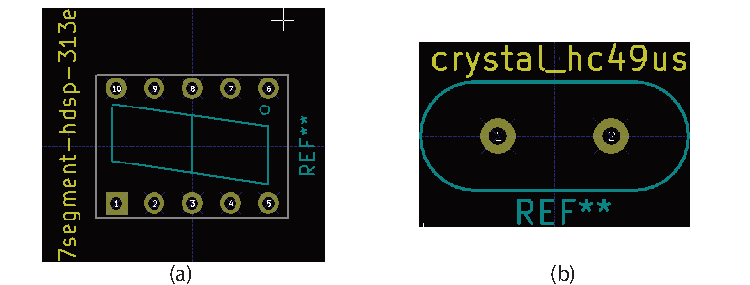
\includegraphics{other-footprints-final}
		\caption{Completed footprints for the (a) HDSP-313E 7-segment LED display and HC-49US 16\,MHz crystal.}
		\label{fig:other-footprints-final}
	\end{figure}

Lastly, we will use the ``Pin\_Headers$\rightarrow$Pin\_Header\_Straight\_1x02'' as the footprint for the 1x2 pin-header connector. 

Now having finished building and selecting all the footprints, we need to go back to CvPcb (Sec.~\ref{sec:cvpcb}) to make the footprint associations. Fig.~\ref{fig:cvpcb-final} shows a screenshot of the completed association. After you are satisfied with the association, click the ``Save'' button and CvPcb will save the footprint assignment into the ``Footprint'' field of the schematic symbols. In fact you can directly add footprint information when you are editing or creating schematic symbols. Nevertheless it is a good idea to run CvPcb to check the association is correctly assigned. 

	\begin{figure}[h]
		\centering
		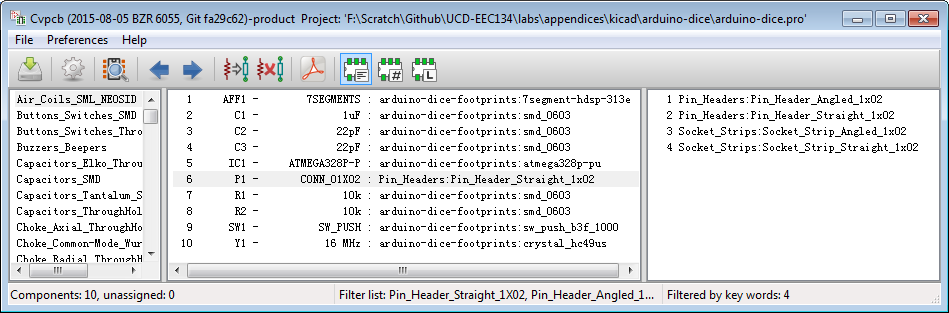
\includegraphics[width=6in]{cvpcb-final}
		\caption{Final schematic symbol and footprint association in CvPcb.}
		\label{fig:cvpcb-final}
	\end{figure}

\subsection{Laying out the PCB}
\label{sec:pcb-layout}

\begin{enumerate}
	\item In Eeschema, double check that the newly assigned footprint information appears in the ``Footprint'' field of the schematic components. Click the ``Generate netlist'' button to generate a netlist file. Simply use the default file name and location. 
	\item Start Pcbnew. 
	\item Click the ``Read Netlist'' button. The ``Netlist'' dialog box will appear. 
		\begin{enumerate}
			\item Click the ``Browse netlist files'' button, and choose the netlist file generated from Eeschema. 
			
			\item Click the ``Read Current Netlist'' button. If the schematic and footprint association has been done properly, you should see no error messages. Otherwise, the Netlist dialog box would complain about missing footprint(s). 
			
			\item If there is indeed no error, close the Netlist dialog box. 
		\end{enumerate}
	\item You should now see a bunch of footprints appear in the Pcbnew main window (Fig.~\ref{fig:ratsnest}). The electrical connections between the components are shown as thin white lines. This initial blob of footprints and lines are often called a ``rat's nest''. 
		\begin{figure}[ht]
			\centering
			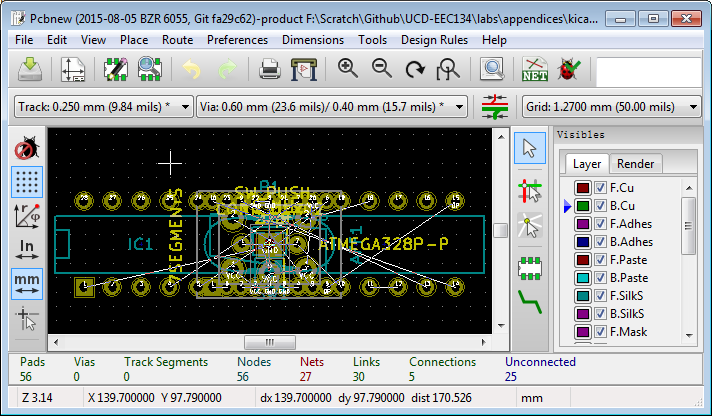
\includegraphics[width=4in]{ratsnest}
			\caption{``Rat's nest'' of footprints and connections after initial import of the netlist.}
			\label{fig:ratsnest}
		\end{figure}	
	
	\item Now move the components into the layout area. Do do this, you can:
		\begin{enumerate}
			\item Right click on a footprint, select the name of the component from the pop-up menu, select ``Move'' from the secondary menu, move your cursor to the desired location and click to finish the move operation. Alternatively, you can mouse over a footprint, press the ``m'' shortcut key, move the cursor to the desire location, and click to finish the move operation. 
			
			\item When a footprint are sitting on top of other footprints, the above operation may become ambiguous because KiCad does not know which footprint you want to select. In such case, a pop-up menu will appear for you select your desired component. 
				\begin{figure}[h]
					\centering
					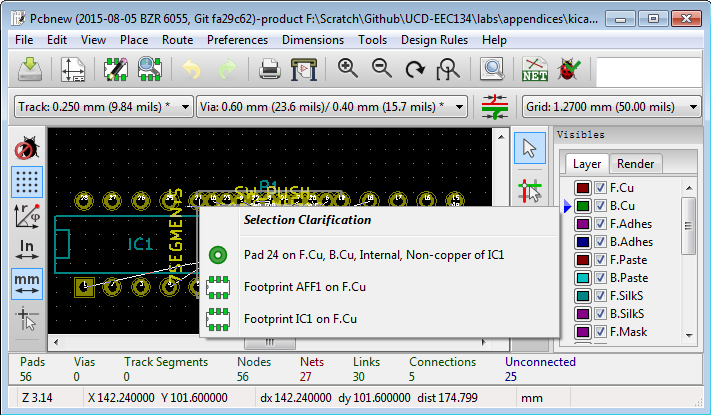
\includegraphics[width=4in]{ambiguity}
					\caption{Component selection ambiguity.}
					\label{fig:ambiguity}
				\end{figure}
			
			\item Let's tentatively arrange the components as shown in Fig.~\ref{fig:layout-iniital}. 
				\begin{figure}[hp]
					\centering
					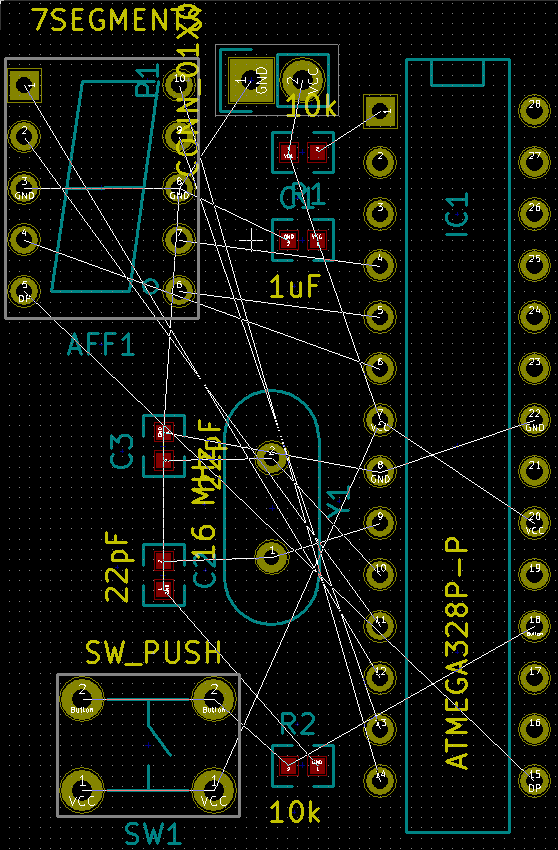
\includegraphics[width=2.5in]{layout-initial}
					\caption{Component arrangement for the Arduino dice PCB.}
					\label{fig:layout-iniital}
				\end{figure}
		\end{enumerate}
		
	\item For this example, we will layout a two layer board, which is the default setting in KiCad. If you need to route more than two layers, you can set it up in ``Design Rules $\rightarrow$ Layers Setup''. In the dialog box that pops up, you can choose from one of the pre-set layer settings provided by KiCad or create your own. KiCad is able to handle up to 32 layers of copper. 

	For the default two-layer board, Table.~\ref{tab:pcb-layers} explains the funtions of each layer. The blue arrow to the left of the layer name indicates the current layer that you are working on. You can turn the visibility of the layers on and off by checking and un-checking the boxes to the right. 
			
		\begin{table}[hp]
			\centering
			\caption{Layers in Pcbnew.}
			\renewcommand{\arraystretch}{1.2}
			\small
			\begin{tabular}{|>{\centering\bfseries}m{1in}|>{\centering\bfseries\arraybackslash}m{4in}|}
				\hline
				Layer name & Function \\
				\hline
				\hline F.Cu & Front side copper trace\\
				\hline B.Cu & Back side copper trace \\
				\hline F.Adhes & Front side adhesives layer. Used to hold SMD components in place during reflow or wave soldering; this layers is used for mass production only. \\
				\hline B.Adhes & Back side adhesives layer.\\
				\hline F.Paste & Opening for front side solder paste. This layer is used to create the solder paste stencils. The solder paste layer openings are usually slightly larger than the pad openings.\\
				\hline B.Paste & Opening for back side solder paste.\\
				\hline F.SilkS & Front side silkscreen printing layer. \\
				\hline B.SilkS & Back side silkscreen printing layer. \\
				\hline F.Mask &	Front side solder mask layer. \\
				\hline B.Mask & Back side solder mask layer. \\
				\hline Edge.Cuts & Circuit board outline drawing.\\
				\hline 
			\end{tabular}
			\label{tab:pcb-layers}
		\end{table}
	
	\item Before we start the actual routing of the circuit traces, let's set up the layout constraints. These constraints usually represent the manufacturing limitations of the PCB manufacturer. For example, Table.~\ref{tab:pcb-parameters} lists typical process parameters from two PCB vendors that we (UC Davis students and researchers) often use. 
		
		\begin{table}[h]
			\centering
			\caption{PCB fabrication process parameters for two PCB vendors.}
			\renewcommand{\arraystretch}{1.2}
			\small 
			\begin{tabular}{|>{\centering\bfseries}m{2in}|>{\centering}m{1.5in}|>{\centering\arraybackslash}m{1.5in}|}
				\hline
				 & \bf Bay Area Circuit student special &  \bf OSH Park \\
				\hline
				\hline Layers & 2 & 2\\
				\hline Substrate material & FR-4 & FR-4 \\
				\hline Substrate thickness & 62\,mil & 62\,mil \\
				\hline Copper thickness & 0.5\,oz & 1\,oz\\
				\hline Minimum Trace Width/ Minimum Spacing & 5\,mil & 6\,mil \\
				\hline Minimum Hole Size &  15\,mil (drill); 5\,mil (annular ring width) & 13\,mil (drill); 7\,mil (annular ring width) \\
				\hline Finish & HASL (tinned) & ENIG (thin gold)\\
				\hline Solder mask color & Green  & Purple\\
				\hline Silkscreen color & White & White\\
				\hline
			\end{tabular}
			\label{tab:pcb-parameters}
		\end{table}		
	
	\item To set up the constraints, go to ``Design Rules$\rightarrow$Design Rules''. A dialog box should appear. 
	\begin{enumerate}
		\item In the ``Global Design Rules'' tab:
			\begin{enumerate}
				\item 	In the ``Minimum Allowed Values'', set the minimum track width, via drill diameter, and via drill diameter (via diameter + 2$\times$annular ring width) according to  Fig.~\ref{fig:design-rules}a. We won't use micro-via settings in this tutorial so their contraints are arbitrarily set.
				\begin{figure}[h]
					\centering
					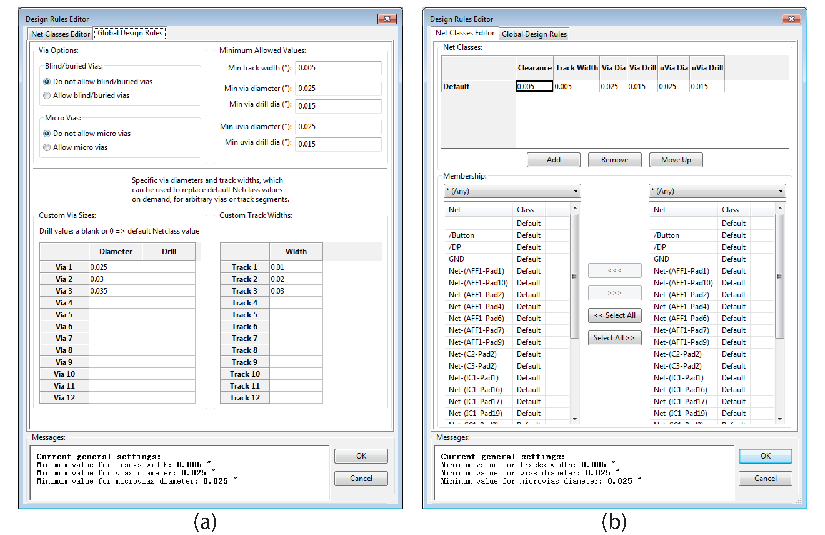
\includegraphics[width=5.5in]{design-rules}
					\caption{Design rules set up.}
					\label{fig:design-rules}
				\end{figure}
				
				\item In this dialog box, you can also set up a list of trace widths and via sizes that you can use in the layout. The above figures shows an example of a list of 10\,mil, 20\,mil, and 30\,mil traces. When you do the layout, these trace widths and via diameters can be selected from drop down menus in the top toolbar.					
			\end{enumerate}
		\item In the ``Net Class Editor'' tab, set the default net class constraints according to Fig.~\ref{fig:design-rules}-b. 	
	\end{enumerate}

	\item Now follow the guidance of the rat's nest lines and connect the components together using copper traces. To draw a trace, you can either:
		\begin{enumerate}
			\item Click the ``Add tracks and vias'' button , click on the component pin that you want the trace to start from, move the cursor to the pin that you want the trace to end, and double click to complete the trace. Alternatively, press the ``x'' shortcut key to start drawing traces, click on the component pin that you want the trace to start from, then move the cursor to the pin that you want the trace to end, and double click to complete the trace.
			
		\end{enumerate}
	\item To add vias, you must start a trace first, then press ``PageDown'' to add a via to the next layer down, or ``PageUp'' to add a via to the next layer up. 
	
	\item Expect a lot of going back and forth between layout the traces and placing the components. 
	
	\item It is often a good practice to fill the PCB with copper to increase the isolation between components and provide easy access to ground. 
		\begin{enumerate}
			\item Click the ``Add filled zones'' button. The next steps will define a rectangular boundary for the copper fill. 
			
			\item Click on a starting point for the fill zone (i.e. one corner of the rectangle). A dialog box should appear. 
			
			\item We'll fill the top layer first so select the ``F.Cu'' from the ``Layer'' list. Select ``GND'' from the ``Net'' list; this will assign GND to the filled copper. Leave everything else as default; you can play with the different settings later on your own. Click ``OK''.
			
			\item Now draw the outline of the fill area. It can be an arbitrarily shaped polygon, but we'll make it a rectangle here. Double click on the starting point to complete the drawing. 
			
			\item Within the area that you've drawn above, right click and select ``Fill or Refill All Zones'' to complete the copper fill. 
			
			\item You can repeat the above steps to do a copper fill for the back side of the PCB. 
			
			\item \textbf{Tip:} When you intend to do a copper fill that is connected to ground, you can actually leave most of the GND terminals (nets) unconnected while laying out the circuit. They will be automatically connected to the nearest copper fill, which is connected to ground. Same thing could be said for VCC terminals if you intend to do a copper fill connected to VCC. 
						
		\end{enumerate}
	
	\item In the last step we will generate the outline of the PCB. This is the physical boundary of the PCB. Fig.~\ref{fig:pcb-outline-example} illustrates an example PCB with a non-rectangular outline. 
		\begin{figure}[hp]
				\centering
				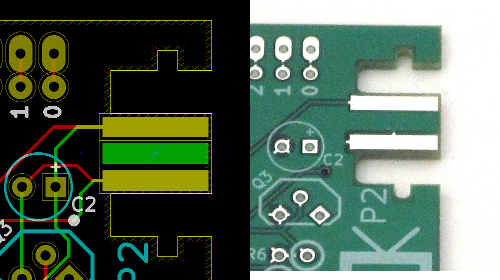
\includegraphics[width=3.5in]{pcb-outline-example}
				\caption{An example of a PCB outline. Source: \href{https://www.wayneandlayne.com/blog/2013/02/26/kicad-tutorial-pcb-edges/}{Link.}}
				\label{fig:pcb-outline-example}
		\end{figure}
	
	To add the board outline:
		\begin{enumerate}
			\item Select the ``Edge.Cuts'' layer. In KiCad, the ``Edge.Cuts'' layer is reserved for the board outline. 
			
			\item It may be helpful to switch to the full-screen cursor mode by toggling the ``Change cursor shape'' button from the left-side toolbar. In the full-screen mode, the horizontal and vertical lines of the cursor extends all the way across the screen, making it easier to find out the board outline that enclose all your layout. 
			
			\item Use the ``Add graphic line or polygon'' tool from the right-side toolbar to draw the board outline. 
		\end{enumerate}
			
	\item Fig.~\ref{fig:layout-final} shows a layout that I produced in the end. 
	
	\begin{figure}[hp]
		\centering
		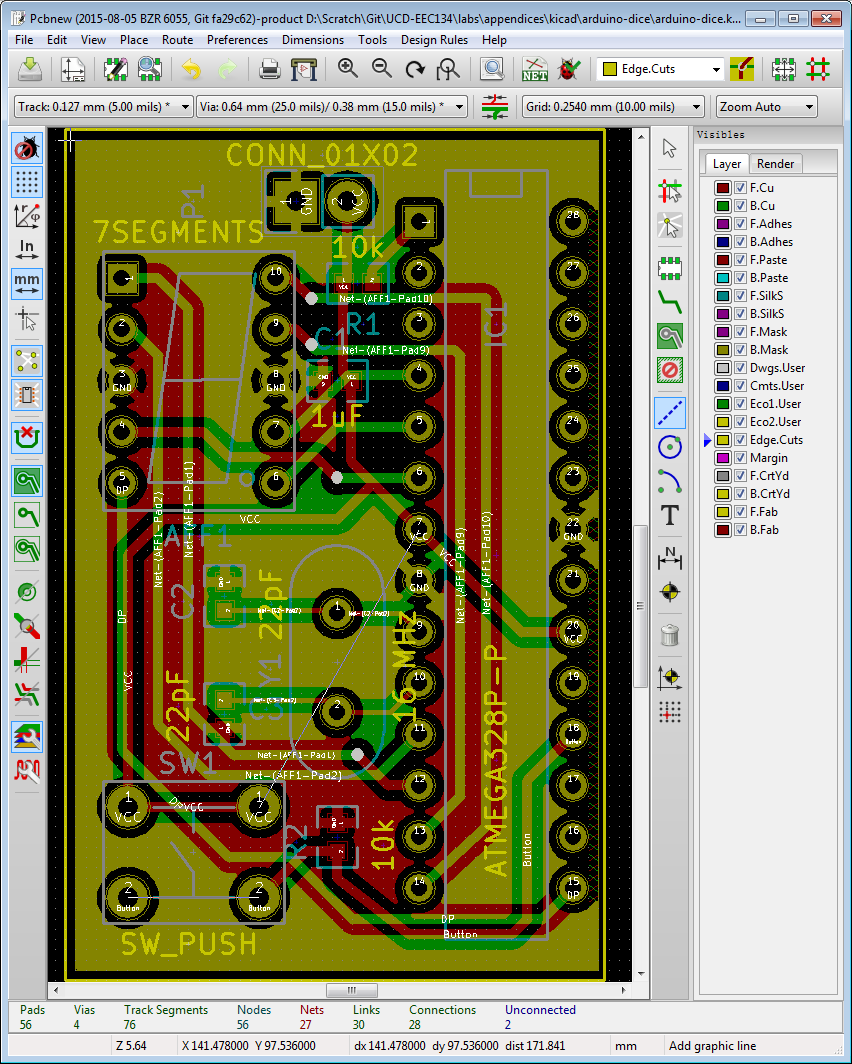
\includegraphics[width=3.5in]{layout-final}
		\caption{Final layout of the Arduino dice PCB.}
		\label{fig:layout-final}
	\end{figure}
\end{enumerate}

\subsection{Generating Fabrication Files}
\label{sec:gerber}

%TODO: add discussion on the different output options 
%e.g.: https://forum.kicad.info/t/what-if-silkscreen-info-is-running-over-copper-islands/123



\begin{enumerate}
	\item After you are satisfied with the PCB layout, you need to generate the artwork files for the PCB manufacturer to produce your PCB. The most common artwork file format is the Gerber format. 
	
	\item To generate the gerber files in Pcbnew, go to ``Files$\rightarrow$Plot''. A dialog box should appear. For most PCB houses, the necessary files include: \emph{F.Cu}, \emph{B.Cu}, \emph{F.SilkS}, \emph{B.SilkS}, \emph{F.Mask}, \emph{B.Mask}, and \emph{Edge.Cuts}. 

	%\item You can use the \emph{F.Paste} and \emph{B.Paste} layers to generate solder paste stencils. 
	
	\item Click ``Plot'' to generate the gerber files for the artwork and click ``Generate Drill File'' to generate the drill file (.drl) for the vias. 
		\begin{figure}[hp]
			\centering
			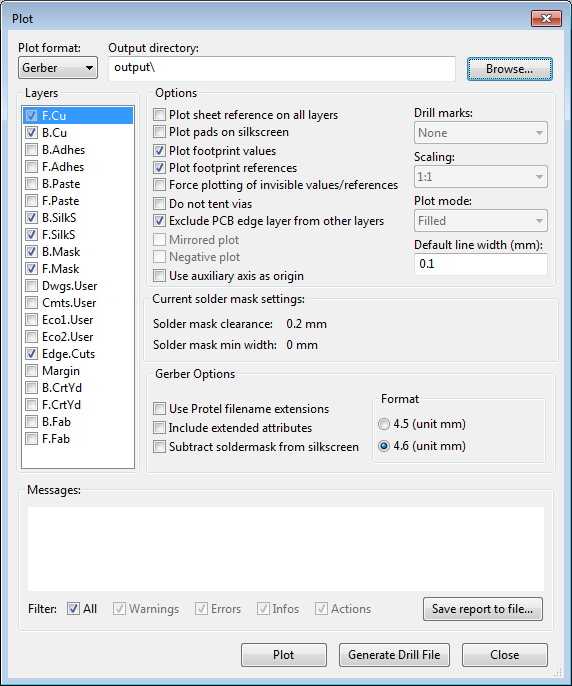
\includegraphics[width=4.5in]{generate-gerber}
			\caption{The ``Plot'' dialog box in Pcbnew.}
			\label{fig:generate-gerber}
		\end{figure}
		
\end{enumerate}

\newpage
\section{Example 2: RF amplifier}

%Under construction. 

In this example, we will explore high frequency PCB designs. We will design a test PCB for the Analog Devices \href{http://www.analog.com/media/en/technical-documentation/evaluation-documentation/ADL5602.pdf}{ADL5602 RF/IF gain block IC}. The ADL5602 has a fixed nominal gain of 20\,dB over a fairly wide frequency range of 50\,MHz--4\,GHz\footnote{If you look at the datasheet carefully, you can see that the gain does fluctuate within a 2\,dB range over the specified frequency range.}. Both the input and output ports of the ADL5602 are internally matched to \SI{50}{\ohm}, making it easier to use this IC as no external matching circuits are needed. 

	\begin{figure}[h]
		\centering
		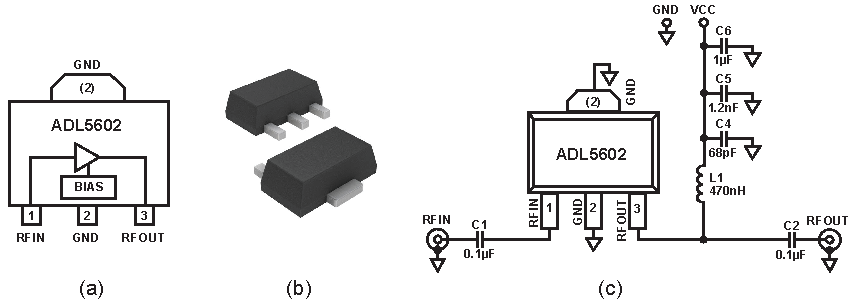
\includegraphics[width=6in]{adl5602}
		\caption{The ADL5602 RF gain block IC. (a) Functional block diagram. (b) Picture of the package. (c) Basic peripheral circuit. Source: ADL56032 datasheet.}
		\label{fig:adl5602}
	\end{figure}

RF IC vendors usually provides suggestions on the peripheral circuit schematic and layout of their ICs. In the case of the ADL5602, the vendor does a good job in providing the recommended circuit connections (Fig.~16 of the datasheet), land pattern (Fig.~17 of the datasheet), and an example layout (Fig.~19 of the datasheet). Note that Fig.~19 of the datasheet is actually the layout for the evaluation board. If you have read enough datasheets, you will realize that an evaluation board is really an example of the recommended layout of the IC's peripheral circuit. Needlessly to say, when you do your own design, you should follow these vendor recommendations as much as you can, unless you really know what you are doing. 

We will follow the evaluation board's design and reproduce it in KiCad. A few modifications are needed for the design to work for our PCB vendor. But before we delve into the design details, we need to understand a few key concepts.

\subsection{Some Unique Concepts to High Frequency PCB Design}

\subsubsection{Controlled Impedance Lines}\label{sec:tline}

Hopefully by this time you have learned enough about RF design to realize that impedance matching is very important at high frequencies ($>$ a few hundred MHz)\footnote{If not, please do review Lecture 2b on transmission lines.}. In general, any trace that carries high frequency signal should be treated as a \textit{transmission line} and its \textit{characteristic impedance} must match those of the source and load impedances to minimize loss due to reflections. 

In the majority of RF systems, all components are matched to a common system impedance of \SI{50}{\ohm}. Therefore, RF signal traces must have a constant impedance all along. This is why transmission lines are also called \textit{controlled impedance lines} in the PCB design world. 

Several forms of transmission lines are amenable for PCB implementation. These include the ``microstrip line,'' the ``strip line,'' and the ``coplanar waveguide (CPW)'' (Fig.~\ref{fig:tlines}-a--c). A variation of the CPW adds a ground plane on the bottom side of the substrate, and can be considered as a combination of microstrip line and a CPW (Fig.~\ref{fig:tlines}-d). We call it ``CPW over ground (CPWG)'' or ``conductor backed CPW (CBCPW)''. 

	\begin{figure}[h]
		\centering
		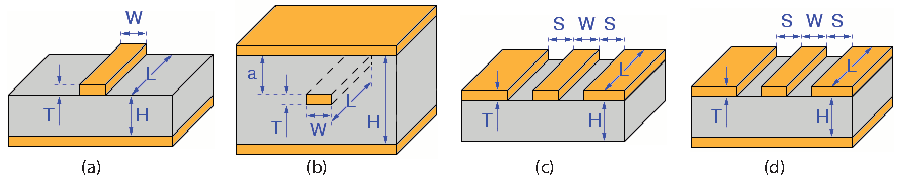
\includegraphics[width=6in]{tlines}
		\caption{Common PCB transmission line implementations. (a) Microstrip; (b) Stripline; (c) CPW; (d) CPWG. Pictures are taken from KiCad's PCB calculator.}
		\label{fig:tlines}
	\end{figure}
	
The impedance of the above transmission lines are determined by their cross-section geometry only. Therefore, to maintain a constant impedance, the cross-section geometry of a trace must remain constant. Some PCB vendors publicize their ability to control line impedance accurately; it is basically another way of saying that they can control the pattern accuracy well. 

Synthesizing the transmission line geometry for a particular impedance is a subject that has been well studied. In fact there are numerous computer programs nowadays that can help you do the job. In this example, we will use an open-source one called \href{http://wcalc.sourceforge.net/}{\textit{Wcalc}}. A similar tool exist under the ``TransLine'' tab within KiCad's PCB calculator tool. 

Microstrip lines are the most commonly used transmission lines on a PCB. The impedance of a microstrip line is primarily determined by its trace width, substrate dielectric constant, and the thickness of the substrate. The metal thickness has a minor effect on the impedance. It is worth noting that the impedance of a microstrip line varies with frequency. However, narrow-band operation, this variation is relatively small and can often be ignored. For circuits that have instantaneous bandwidth spanning multiple GHz, this frequency dependent impedance variation needs to be investigated.  

The loss of the transmission line is primarily determined by the loss tangent of the substrate. For circuits operating above a few GHz, low-loss substrates, such as the Rogers Duroid 5880 and 4350, are usually preferred. These substrates tend to be more expensive, in terms of both procurement and fabrication. 

In the ideal case, the RF PCB designer can choose the optimal substrate stack-up to achieve the best high frequency performance. In a less-than-ideal case, other factors may come into play. For low-GHz range, for example, cost usually dominates the selection of substrate and low-cost substrates such as the FR-4 are more common, although they do not have great loss characteristics. In the case of EEC 134 designs, we are bound to using low-cost PCB vendors whose only offerings are on FR-4 substrates with a fixed thickness. 

So the only variable left to us is the trace width. Using the specifications of Bay Area Circuits (substrate thickness = 62\,mil, substrate dielectric constant = 4.8\footnote{Note that these constraints apply only to student special bundles.}), we can synthesize the trace width needed for a \SI{50}{\ohm} impedance using Wcalc. It turns out to be 108\,mil, or 2.74\,mm (Fig.~\ref{fig:ustrip-synth}). This is quite large! As a comparison, the smallest pin width of the ADL5602 chip is only 0.32--0.52\,mm. The separation between the input and output pins is 3\,mm, not much bigger than 2.74\,mm. Obviously it would be quite difficult to layout the circuit with such a wide trace. 

	\begin{figure}[h]
		\centering
		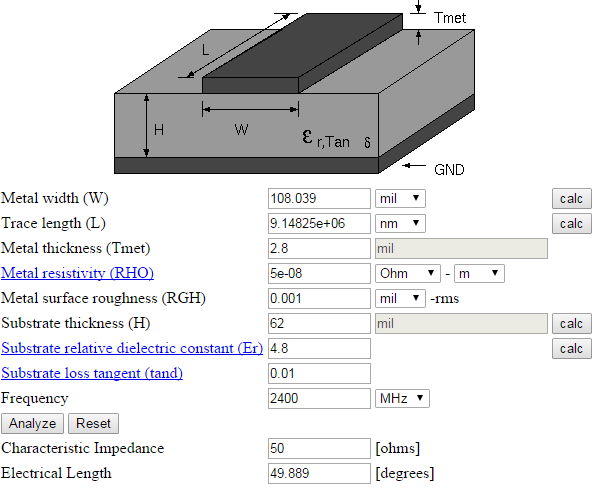
\includegraphics[width=4in]{ustrip-synth}
		\caption{Synthesizing a \SI{50}{\ohm} microstrip line with Wcalc.}
		\label{fig:ustrip-synth}
	\end{figure}

One trick we can play to reduce the trace width is to use the CPWG configuration. Compared with the microstrip, the CPWG adds two coplanar ground planes which increases the capacitance per unit length $C'$ of the transmission line. An increased $C'$ means that the center conductor trace width can be reduced. In addition, the separation between the center conductor and the coplanar ground planes can be adjusted to further increase $C'$.  

The minimum trace separation allowed by Bay Area Circuits is 5\,mil. If we allow some tolerance on it and use 6\,mil as the separation, we could synthesize the required center conductor width using Wcalc. For a \SI{50}{\ohm} transmission line, this width is 37\,mil, or 0.94\,mm (Fig.~\ref{fig:cpwg-synth})\footnote{Note that the transmission line length and copper thickness have a negligible effect on the line impedance.}. Although it's still quite a bit larger than the ADL5602 pin size, it's much better than that of the microstrip case. 

	\begin{figure}[hp]
		\centering
		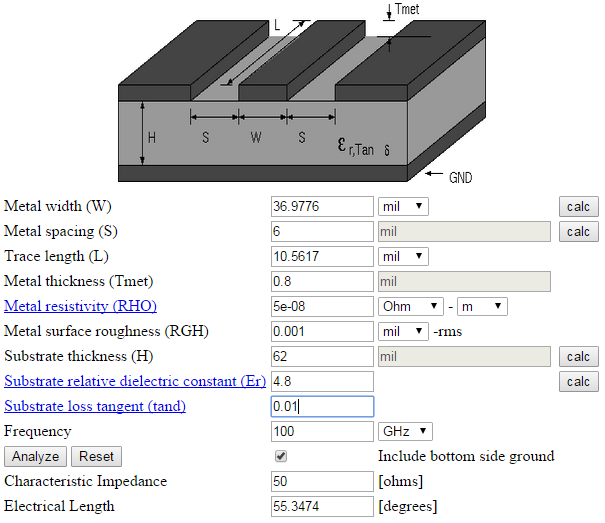
\includegraphics[width=4in]{cpwg-synth}
		\caption{Synthesizing a \SI{50}{\ohm} CPWG line with Wcalc.}
		\label{fig:cpwg-synth}
	\end{figure}

To implement a CPWG on a PCB, it is critical to connect the three (two on the top plus the bottom) ground planes together. This is usually done with vias. Fig.~\ref{fig:cpwg-example} shows an example of CPWG design on a PCB. Later in this tutorial, we will show you how to implement it in KiCad. 

	\begin{figure}[hp]
		\centering
		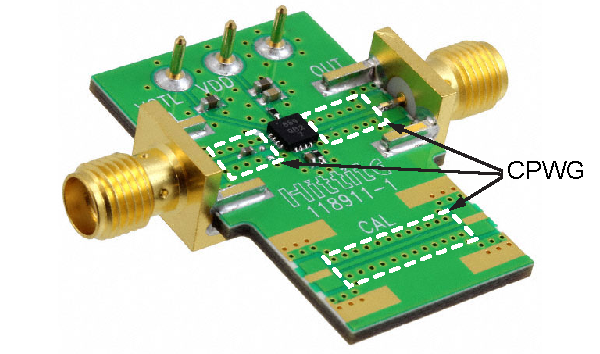
\includegraphics[width=3in]{cpwg-example}
		\caption{CPWG on a Hittite Microwave evaluation board.}
		\label{fig:cpwg-example}
	\end{figure}

\newpage
\subsubsection{Microstrip lines with Top Copper Shield}

One of the many challenges in RF PCB design is to provide good isolation between signals of different frequencies and strength. The contention and interference between signals may come from desired or undesired sources. For example, in RF transceivers, we are often dealing with very weak signals coming into the receiver whereas a transmitting signal several tens of dB stronger may be right close by on the same PCB. Another example exists in many digital processors with high clock speed as they tend to generate ample high frequency (up to a few GHz) noise due the sharp rising and falling edges of the digital signals. 

One of the techniques for providing good isolation at high frequencies is to shield the signal traces with ground planes and row(s) of vias.  Fig.~\ref{fig:via-fence} shows an example PCB employing such a technique. The ``via fence'' and the top ground plane effectively serve as a cage to contain the RF signal traveling on the microstrip line to prevent it from affecting or being affected by other signals. To be effective, the distance between adjacent vias should be much smaller than a wavelength. 

	\begin{figure}[hp]
		\centering
		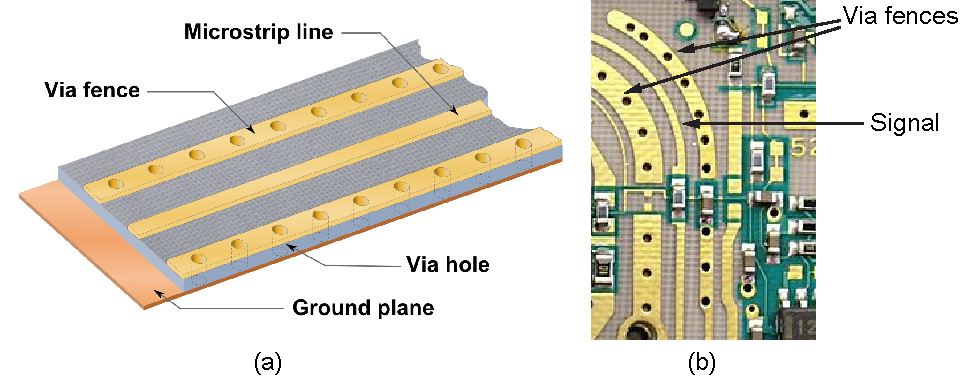
\includegraphics[width=5.5in]{via-fence}
		\caption{Via fences and top ground plane shields for microstrip lines. Source: \href{https://en.wikipedia.org/wiki/Via_fence}{Wikipedia}.}
		\label{fig:via-fence}
	\end{figure}

While Fig.~\ref{fig:via-fence} shows islands of shielding structures, many PCB designers opt to fill the entire signal layer with ground plane and vias. This is usually called ``copper fill'' or ``copper pour'', and has been discussed in Example 1. 

The acute reader will have noticed that the CPWG on PCB (Fig.~\ref{fig:cpwg-example}) inherently has rows of vias to act as shields and in fact it looks rather similar to the microstrip line with via fence shields (Fig.~\ref{fig:via-fence}). So what exactly is the difference between the two designs?

In principle, there is not much of a difference; both designs are planar transmission lines with ground planes and vias serving as shields. In practice, the biggest distinction is the separation or gap $S$ (Fig.~\ref{fig:tlines}) between the signal trace and the coplanar ground planes. In a CPWG, $S$ is small and contributes significantly to the $C'$ of the transmission line whereas in a shielded microstrip, $S$ is large and its effect on the line impedance is kept small. \textit{A rule of thumb is that $S$ needs to be larger than two or three times the width of the signal trace for a shielded microstrip.} In a CPWG, $S$ must be chosen carefully to get the right impedance. 

\subsubsection{Transmission Lines Bends}

To maintain a nice constant impedance along the transmission line, it is desirable to maintain a constant cross-section geometry. In a complex circuit, however, you may often need to route the high frequency signal to different directions, depending on the orientation and alignment of the circuit components. When the signal trace changes direction, the cross-section inevitably needs to change at the bend, resulting in some impedance perturbation. For a right angle bend of a microstrip line, for example (Fig.~\ref{fig:bends}-a), the corner section effectively has a larger width and it results in an extra shunt capacitance. In addition, due to the skin effect, high frequency signals on a planar transmission line tend to travel on the edges of the trace. As the signal passes through the bend, the current/voltage wave on the outer edge of the bend has to travel a longer distance than the wave on the inner edge. This additional length effectively results in an extra series inductance. The extra capacitance and inductance creates a low-pass frequency response and limits the bandwidth of the transmission line. 

	\begin{figure}[hp]
		\centering
		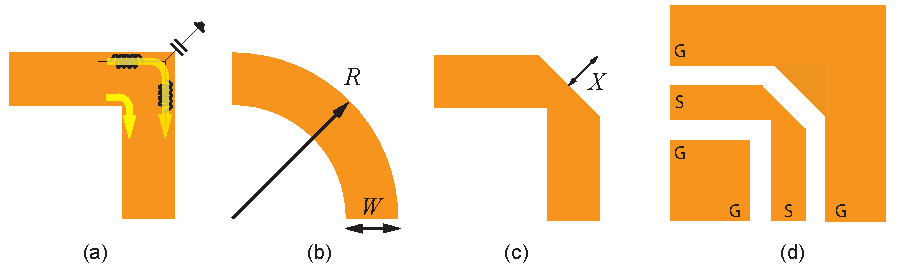
\includegraphics{bends}
		\caption{(a) Effects of a right angle bend on the microstrip line characteristics. (b) A microstrip circular bend. (c) A microstrip mitered bend. (d) A CPW mitered bend.}
		\label{fig:bends}
	\end{figure}

To overcome the adverse effects of a transmission line bend, several bending structures can be employed. A circular bend (Fig.~\ref{fig:bends}-b) smooths out the impedance discontinuity and is often used when board area is not of a major concern. \textit{The rule of thumb here is that the radius $R$ of the bend should be larger than three times the line width $W$.}

Fig.~\ref{fig:bends}-c\&d show another strategy; the corner of the bend is cut off abruptly to mitigate the extra capacitance and inductance. This is called a ``mitered bend''. The optimal design of a mitered bend has been studied thoroughly in the 1970s\footnote{R.J.P. Douville and D.S. James, Experimental Characterization of Microstrip Bends and Their Frequency Dependent Behavior, 1973 IEEE Conference Digest, October 1973, pp. 24-25. \\
R.J.P. Douville and D.S. James, Experimental Study of Symmetric Microstrip Bends and Their Compensation, IEEE Transactions on Microwave Theory and Techniques, Vol. MTT-26, March 1978, pp. 175-181.}. An empirical equation for the cut depth $X$ is given by \textit{Douville} and \textit{James}

\[
X = \frac{W}{\sqrt{2}} \left\{0.52 + 0.65e^{ -1.35\frac{W}{ H}}    \right\}
\]
where $H$ is the thickness of the substrate. This formula is valid for $0.25\leq W/H \leq 2.75$. 

With the availability of many powerful electromagnetic simulators, it is probably best to simulate the structure to ensure the best performance for a particular PCB stack-up. But doing so may also be an overkill for non-critical designs. The bottom line is that paying attention to the bend structure is probably better than doing nothing!

\subsubsection{Short transmission lines}\label{sec:short-tline}

In previous sections and whatever RF courses you have taken, we have learned that it is very important to maintain good impedance matching on signal traces that carry high frequency signals. New students to the world of high frequency electronics tend to follow the impedance matching principle dogmatically. However, we will see in this subsection that there are certain cases when you don't need to worry about impedance matching too much!

Let's consider a transmission line of characteristic impedance $Z_t$ and length $l_t$, connected to a load impedance of $Z_0$. We know that the input impedance looking into the transmission line and the corresponding reflection coefficient are given by

\[
Z_{in} = Z_t \frac{Z_0 + j Z_t \tan \beta l_s}{Z_t + j Z_0 \tan \beta l_s},
\]

\[
\Gamma_{in} = \frac{Z_{in}-Z_0}{Z_{in}+Z_0}.
\]

If $Z_t$ is not equal to $Z_0$, then $Z_{in}$ will generally be a complex number that changes with $l_s$. To get a more intuitive feeling for what $Z_{in}$ looks like, we plot $\Gamma_{in}$ for various $Z_t$ and $l_s$ values. 

\begin{figure}[ht]
	\centering
	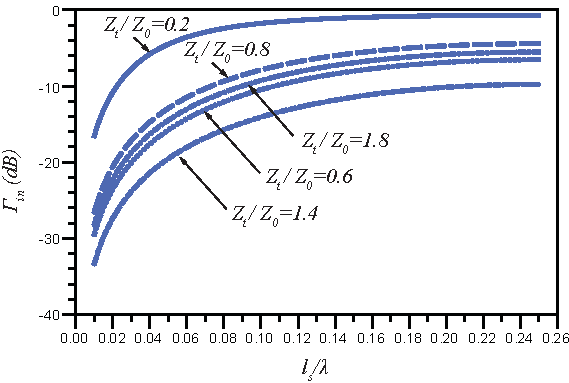
\includegraphics{short-tline-gamma}
	\caption{Reflection coefficients for various $l_s$ and $Z_t$.}
	\label{fig:short-tline-gamma}
\end{figure}

%	\begin{figure}[h]
%		\centering
%		\pstool{short-tline-gamma.eps}{
%			\psfrag{gamma}{test}
%			\psfrag{rL}{$L_s/\lambda$}
%			\psfrag{rZ=0.2}{$Z_t/Z_0=0.2$}
%			\psfrag{rZ=0.6}{$Z_t/Z_0=0.6$}
%			\psfrag{rZ=1.4}{$Z_t/Z_0=1.4$}
%			\psfrag{rZ=1.8}{$Z_t/Z_0=1.8$}
%			\psfrag{rZ=2.0}{$Z_t/Z_0=2.0$}
%		}
%		\caption{Reflection coefficients for various $l_s$ and $Z_t$.}
%		\label{fig:short-tline-gamma}
%	\end{figure}

It is clear from the graph that as $l_s$ approach 0, $\Gamma_{in}$ also approaches 0 ($-\infty$ in dB) regardless of the $Z_t$ value. This is hardly surprising because when $l_s$ is extremely small the transmission line basically vanishes and the input is connected to the matched load directly. If you remember the teachings from EEC 130A\footnote{EEC 130A is the introductory electromagnetics course at UC Davis.}, we consider transmission line effects only when electrical length of a line is appreciable compared to a wavelength. For short electrical connections, we treat them as short circuit. 

This is why controlling the transmission line impedance is not very important for small $l_s$. Exactly how small is considered ``small'' depends on the particular $Z_t$ value and the level of input reflection you can tolerate. In general, it is good practice to keep circuit components as close to each other as possible. 

\subsection{Circuit schematic and component selection}
We will create a project named ``rf-gain-block''. We will follow the circuit given in Fig.~\ref{fig:adl5602}-c for this example PCB design. The schematic capture and schematic symbol creation should be straightforward if you have gone through Example 1. Fig.~\ref{fig:example2-schematic} shows an example schematic capture in KiCad. 

\begin{figure}[hp]
	\centering
	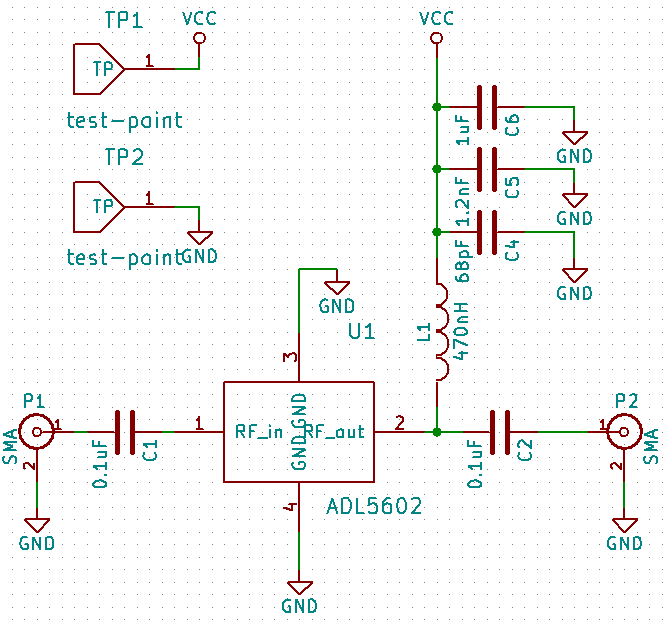
\includegraphics[width=3in]{example2-schematic}
	\caption{Schematic of the ADL5602 example circuit. }
	\label{fig:example2-schematic}
\end{figure}

The datasheet gives a recommended bill of materials (BOM, Table 6 of the ADL5602 datasheet). It is worth noting that C1 and C2, which are the input and output dc-blocking capacitors, have been sized to 0402 (imperial) to match the width of the input and output \SI{50}{\ohm} transmission line. However, the datasheet recommended circuit is built on a different substrate than what we are going to use. From the calculation in Section.~\ref{sec:short-tline}, our \SI{50}{\ohm} CPWG line width is about 37\,mil, which is closer to the width of a 0603 (imperial) component. Therefore, in our design, C1 and C2 are going to be size 0603. Table.~\ref{tab:adl5602-bom} list the modified BOM. 


\begin{table}[h]	
	\renewcommand\arraystretch{1.2}
	\caption{BOM for the ADL5602 Circuit.}
	\begin{tabular}{|c|>\centering m{1.6in}|>\centering m{1.2in}| m{1.4in}|}
		\hline
		\textbf{Component} & \textbf{Description} & \textbf{Default Value} & \textbf{Package} \\
		\hline
		\hline
		C1, C2 & dc-block capacitors & \SI{0.1}{\micro\farad} & 0402 \\
		\hline
		
		L1 & RF-choke inductor & 470\,nH & 0603 (Coilcraft 0603LS-NX or equivalent) \\
		
		\hline
		C4 & power supply decoupling capacitors & 68\,pF & 0603 \\
		
		\hline
		C3 & power supply decoupling capacitors & 1.2\,nF & 0603\\
		
		\hline
		C2 & power supply decoupling capacitors & \SI{1}{\micro\farad} & 0603 \\
		
		\hline
		VCC, GND & power supply & & test pins \\
		
		\hline
		P1, P2 & RF input and output SMA connectors & & SMA \\
		\hline
	\end{tabular}
	\label{tab:adl5602-bom}
\end{table}

\subsubsection{RF-choke inductor}

The L1 inductor serves to provide the dc bias current for the amplifier while preventing the RF signal from going into the low-impedance dc source (VCC). It does so by providing a low dc impedance and a high RF impedance, which is consistent with the impedance behavior of an inductor. 

In reality, however, all components have parasitics due to their finite physical size and proximity to other components/circuits. These parasitics can be inductive, capacitive, and/or resistive. Fig.~\ref{fig:ind-equiv} shows a simple equivalent circuit for a realistic inductor, where $R_s$ represents the resistive loss in the inductor and $C_p$ represents the parasitic capacitance between the input and output terminals of the inductors. Because the impedances of inductors and capacitors are frequency dependent, the frequency response of a realistic inductor exhibit more complex behavior than an ideal inductor. 

	\begin{figure}[h]
		\centering
		\begin{circuitikz}
			\draw (0,0) to [short, o-*] (1,0)
			(1,-1) to (1,1)
			(1,1) to [inductor, l=$L_s$] (3,1) to [R, l=$R_s$] (5,1)
			(1,-1) to (2,-1) to [capacitor, l=$C_p$] (4,-1) to (5,-1)
			(5,-1) to (5,1)
			(5,0) to [short, *-o] (6,0);
		\end{circuitikz}
		\caption{A simple equivalent circuit for a realistic inductor.}
		\label{fig:ind-equiv}
	\end{figure}

For example, if $R_s$ is small, $C_p$ will resonant with $L_s$ to create a parallel resonant tank which present a high impedance. The resonant frequency of $C_p$ and $L_s$ is called the self-resonant frequency (SRF). For an RF-choke inductor, this behavior works to our advantage because it enhances the inductor's capability to reject RF signals around the SRF. However, if the operating frequency is too much higher than SRF, $C_p$ starts shorting out the input and output terminals and the impedance of the inductor starts to drop. As an example, Fig.~\ref{fig:ind-impedance} shows the impedance-frequency profile of the Coilcraft 0603LS-471 ceramic inductor that we are going to use in this example. Although the effective inductance starts to drop around 500\,MHz, the impedance reaches a peak around 800\,MHz and is above 200 from 100\,MHz to above 1.5\,GHz.

\begin{figure}[ph]
	\centering
	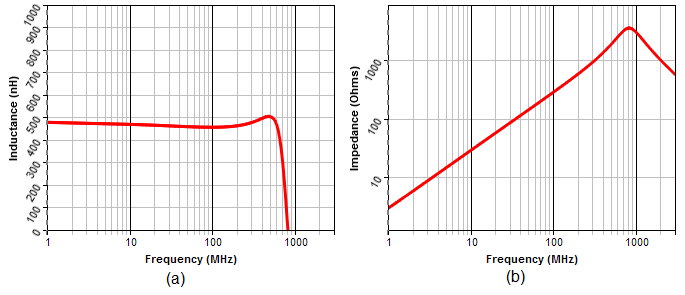
\includegraphics[width=5.5in]{ind-impedance}
	\caption{Impedance profile of the Coilcraft 0603LS-471 inductor. Source: \href{http://www.coilcraft.com/apps/compare/compare_rf.cfm?partlist=0603LS-471}{Link}.}
	\label{fig:ind-impedance}
\end{figure}

\subsection{Component footprints}
Several custom footprints need to be created for this PCB as shown below. All the footprints will be collected in a project footprint library named ``rf-gain-block-footprints''. 

\subsubsection{ADL5602 footprint}

The footprint of the ADL5602 IC will follow its recommended land pattern in its datasheet. It is copied in Fig.~\ref{fig:adl5602-landpattern}-a for easy reference. The large exposed pad in the center and the many vias serve two purposes: 1) providing a low-impedance electrical path to the ground plane underneath; 2) providing a low thermal impedance path so that the heat generated in the IC could be well dissipated. 

\begin{figure}[ht]
	\centering
	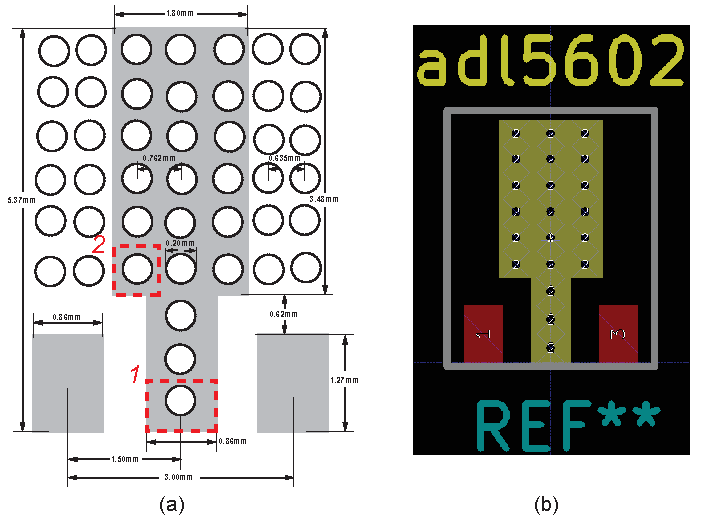
\includegraphics[width=4.5in]{adl5602-landpattern}
	\caption{(a) Datasheet recommended land pattern for ADL5602 IC. Source: ADL5602 datasheet. (b) Footprint in KiCad.}
	\label{fig:adl5602-landpattern}
\end{figure}

Pad 1 and 3 are straightforward to generate in KiCad. The creation of pad 2, the large ground pad, requires a little bit of guidance. Our strategy here is to draw each via as a separate pad with rectangular pad area and a circular drill. The complex land pattern consists of two unit cell types, both labeled  in Fig.~\ref{fig:adl5602-landpattern}-a. Pad type 1 has a width of 0.86\,mm and a height of $(0.62+1.27)/3=0.63$\,mm. Pad type 2 has a width of 0.762\,mm and a height of $(5.37-0.62-1.27)/6=0.58$\,mm. The drill diameter for both pad types is 0.20\,mm. 

\begin{enumerate}
	\item In the footprint editor, set the unit to ``mm''.
	\item Place pad type 1 at (0, -0.315). 
	\item Use the array tool to create the rest of the three type 1 pads. 	
		\begin{enumerate}
			\item Right click on the pad created above, select ``Create Pad Array'' (shortcut ``ctrl+N''). Set up the ``Create Array'' dialog box according to Fig.~\ref{fig:pad-array-1}. Leave the numbering settings to their default values.
			
			\begin{figure}[hp]
				\centering
				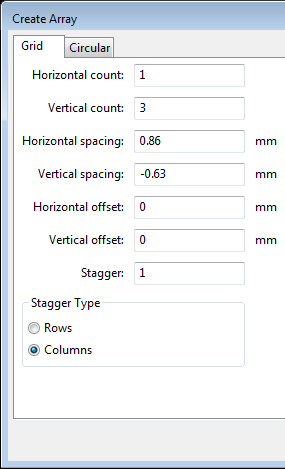
\includegraphics[width=2in]{pad-array-1}
				\caption{Array setting for pad type 1.}
				\label{fig:pad-array-1}
			\end{figure}
			
			\item Now change the pad numbers of the three pads all to 2. You have to do this one by one. It is a pity that KiCad does not allow automatic numbering of an array with a single number. 
			 
		\end{enumerate}
	\item Create the first type 2 pad at (-0.762,-2.18). Following similar steps as above, create a 3$\times$6 array with pad number 2.
	
	\item The final footprint is shown in Fig.~\ref{fig:adl5602-landpattern}-b. A courtyard outline has also been added. 

In the above steps, we have followed the datasheet recommendations faithfully. Sometimes, however, there are other constraints that force you to deviate from the suggested footprint. For example, the Bay Area Circuits Student Special bundle has a minimum drill size of \SI{15}{\micro\meter} which is almost twice as large as the recommended drill size for the vias in the ground pad. As a result, you will not be able to fit as many vias in the ground pad. 

\end{enumerate}

\subsubsection{Inductor footprint}

The Coilcraft 0603LS series inductors have a recommended footprint (copied here in Fig.~\ref{fig:cc-0603ls}-a). Fig.~\ref{fig:cc-0603ls}-b shows the created footprint in KiCad. 

	\begin{figure}[hp]
		\centering
		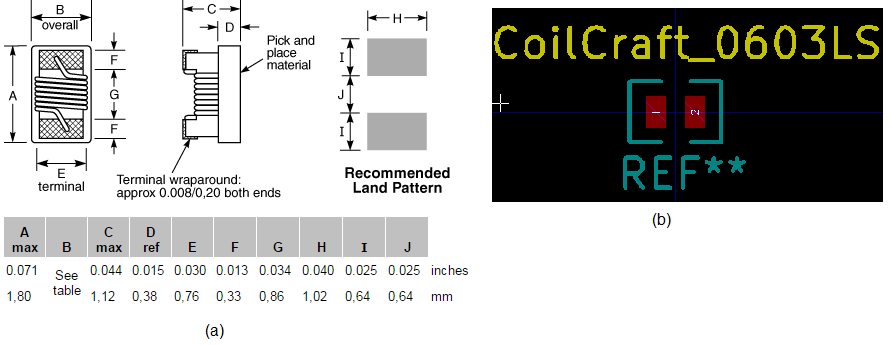
\includegraphics[width=6in]{cc-0603ls}
		\caption{Coilcraft 0603LS series footprint.}
		\label{fig:cc-0603ls}
	\end{figure}

\subsubsection{SMA connector footprint}
The footprint of the SMA connector used in this lab is given in Fig.~\ref{fig:sma-footprint}. 

	\begin{figure}[hp]
		\centering
		\includegraphics[width=5.5in]{sma-footprint}
		\caption{(a) Picture of the SMA end-launch connector. (b) Recommended land pattern. (c) Footprint in KiCad.}
		\label{fig:sma-footprint}
	\end{figure}

\subsubsection{VCC and GND footprint}
The dc power to the circuit is going to be applied through two test points, one for VCC and the other for GND. Fig.~\ref{fig:testpoint-footprint}-a shows a picture of the clip-on test point (\href{http://www.digikey.com/product-detail/en/5001/5001K-ND/255327}{Keystone Electronics 5001}) and its outline drawings. The footprint of this test point is simply a circular pad with a drill diameter of 1.1\,mm and a total diameter of 2\,mm. The 1.1\,mm drill diameter is chosen to be slightly smaller than the widest separation (1.39\,mm) between the two legs of the test point so that when the test point is inserted into the hole, mechanical tension could keep it in place for easy soldering. 

	\begin{figure}[ph]
		\centering
		\includegraphics[width=4.5in]{testpoint-footprint}
		\caption{(a) Picture of the test point and its outline drawings. Source: \href{http://www.digikey.com/product-detail/en/5001/5001K-ND/255327}{Link}. (c) Footprint in KiCad.}
		\label{fig:testpoint-footprint}
	\end{figure}
	
\subsection{PCB Layout}

In designing an RF PCB, we usually start with the layout of the RF components and traces. The traces that carry high frequency signals should be kept as short as possible and as straight as possible. In our design, we will align the input and output RF traces in a straight line and connect the input and output pins of the ADL5602 IC in perpendicular to the RF traces. Fig.~\ref{fig:adl5602-connection} shows the ``ideal'' connection to the ADL5602 IC. The input and output traces are tapered to minimize the coupling between the two. 

In KiCad, however, all traces have a rounded end shape and tapering cannot be easily implemented. A less-than-ideal approach is to use segments of traces of different width to make the connection. In Fig.~\ref{fig:adl5602-connection}-b for example, a 20-mil trace segment is used to bridge the pad and the 37-mil trace\footnote{The 20-mil trace is invisible because it has the same color as the pad and the 37-mil trace.}. 

In the actual layout, we try to keep the components as close to each other as possible. As such, it may be difficult to fit the 37\,mil trace in between the components. As discussed in Section~\ref{sec:short-tline}, however, impedance matching is not as important at small length scale and it is OK to connect the components with a thinner trace.

\begin{figure}[ph]
	\centering
	\includegraphics{adl5602-connection}
	\caption{(a) ``Ideal'' PCB connection to the ADL5602 IC. (b) Implementation in KiCad.}
	\label{fig:adl5602-connection}
\end{figure}


The layout of the rest of the circuit should be straightforward. Fig.~\ref{fig:example2-layout-prelim} shows a preliminary layout. Notice that we have placed the RF components along a straight line and have minimized the distance between the components to minimize the insertion and reflection losses. 

\begin{figure}[ht]
	\centering
	\includegraphics[width=3.5in]{example2-layout-prelim}
	\caption{Initial layout of the example 2 circuit.}
	\label{fig:example2-layout-prelim}
\end{figure}

\subsubsection{Copper fill}
At this point, we need to remind ourselves that the 37-mil trace width gives \SI{50}{\ohm} impedance only in a CPWG configuration with a 6-mil gap (Section.~\ref{sec:tline}). To implement the CPWG, we will use the copper fill feature that we introduced in Example 1. 

\begin{enumerate}
	\item Click the ``Add filled zones'' button to turn on the copper fill tool. 
	
	\item Click at the upper left corner of your intended fill region, a dialog box should appear. Set up the parameters as follows: 
		\begin{enumerate}
			\item Net: GND (This sets the electrical connection of the copper fill to ground.)
			
			\item Clearance: 0.006'' (This sets the separation between the trace and the GND-connected copper fill.)
			
			\item Pad connections: Solid (For RF circuit, we usually don't use thermal relief for pads to minimize the inductance/impedance to ground.)
		\end{enumerate}
	\item Draw the outline of the fill zone. The fill zone needs to be a closed region. Double click to finish the drawing. You may find it a lot easier to move the cursor around using the keyboard arrow keys. Repeat this for all metal layers that you want to fill. In this example, both the top and the bottom copper layers will be filled. 
	
	\item Once the fill zones have been defined, right click on anywhere in the main layout window and select ``Fill or Refill All Zones'' to create the copper fill. Fig.~\ref{fig:example2-layout-fill} shows the copper filled layout. Notice that the gap between the trace and the fill is uniform everywhere. This is because we have set up only one fill zone on each layer. Setting up multiple fill zones will allow you to have multiple separations. 
	
\end{enumerate}

	\begin{figure}[ht]
		\centering
		\includegraphics[width=6in]{example2-layout-fill}
		\caption{Layout of the example 2 circuit after copper filling. (a) Front side. (b) Back side. Note that the component footprint is always visible.}
		\label{fig:example2-layout-fill}
	\end{figure}
	
\subsubsection{Via fences}
The last step (before defining board outline) is to create the via fences that connect the top and bottom ground fills. In PCB terminology, this is often called ``via stitching''. Unlike more sophisticated PCB tools, such as Cadence Allegro and Altium Designer, KiCad does not have a dedicated tool for via stitching. However, there are several hacks for implementing it. We will follow a procedure proposed in this \href{https://forum.kicad.info/t/protip-nicer-via-stitching/1103/21}{link}.
	\begin{enumerate}
		\item Open the footprint editor. Select ``rf-gain-block-footprints'' as the active library. 
		
		\item Create a new footprint named ``via-15mil''. Here ``15mil'' indicate the drill diameter of the via. 
		
		\item Insert a pad and set it up as follows: 
			\begin{enumerate}
				\item Pad type: Through-hole
				\item Shape: circular
				\item Size X: 0.030''
				\item Drill$\rightarrow$Size X: 0.015''
				\item Layers$\rightarrow$Copper: All copper layers
				\item Unselected everything under ``Technical layers''. By default, ``F.SilkS'', ``F.Mask'', and ``B.Mask'' layers are selected. In particular, unselecting the ``F.Mask'' and ``B.Mask'' layers ensures that no solder mask openings are created and that we will have vias covered by the solder mask material in the end\footnote{In PCB terminology, such vias are called ``tented vias''.}.  
			\end{enumerate}
		\item Save the footprint. 
		
		\item In the Pcbnew, click the ``Add footprints'' button and click on the main layout window to insert a footprint directly. Select the ``via-15mil'' footprint and place it along the edges of the copper fill. For via fences around RF traces, a rule of thumb is to set the via spacing no larger than 1/20th of the propagation wavelength. Obviously you also need to make sure that the via spacing is not too small as to violate the design rules of the PCB manufacturer. Fig.~\ref{fig:example2-layout-via} shows the layout after the via stitching. 
		
		\begin{figure}[ht]
			\centering
			\includegraphics[width=3.5in]{example2-layout-via}
			\caption{Layout of the example 2 circuit after via stitching.}
			\label{fig:example2-layout-via}
		\end{figure}
		
	\end{enumerate}

We have now completed the second example. 

%TODO: an example showing high speed digital circuit
%\section{Example 3: High speed digital board}
% differential pair

\newpage
\section{Further Reading}

* Not in any particular order. 

\begin{itemize}
	\item \href{http://www.edn.com/electronics-blogs/the-practicing-instrumentation-engineer/4418080/2/Shields-are-your-friend--except-when-}{Shields are your friend, except when...}, (\href{http://www.edn.com/electronics-blogs/the-practicing-instrumentation-engineer/4419228/2/Shields-are-your-friend--except-when---Part-2-}{Part 2}), (\href{http://www.edn.com/electronics-blogs/the-practicing-instrumentation-engineer/4420553/Shields-are-your-friend--except-when---Part-3-}{Part 3}).
	
	\item KiCAD keyboard PCB design guide: \url{http://deskthority.net/wiki/KiCAD_keyboard_PCB_design_guide}{}

	\item Online KiCad footprint generator: \url{http://kicad.rohrbacher.net/quickmod.php}

	\item KiCad library management strategies: \url{https://docs.google.com/document/d/1M38ByFyqnhwGo8b_jDDyBceyZtEGeaSAuQaP9REzWrU/edit}

	\item KiCad footprint management (somewhat outdated):
\url{http://mithatkonar.com/wiki/doku.php/kicad/footprint_management}

\end{itemize}

\end{document}
